\chapter{The Tree That Grew Triangles}



\bigskip\centerline{\rule{0.5\textwidth}{0.4pt}}\bigskip



\section*{A Puzzle for the Pharaohs}

\begin{figure}[htbp]
\centering
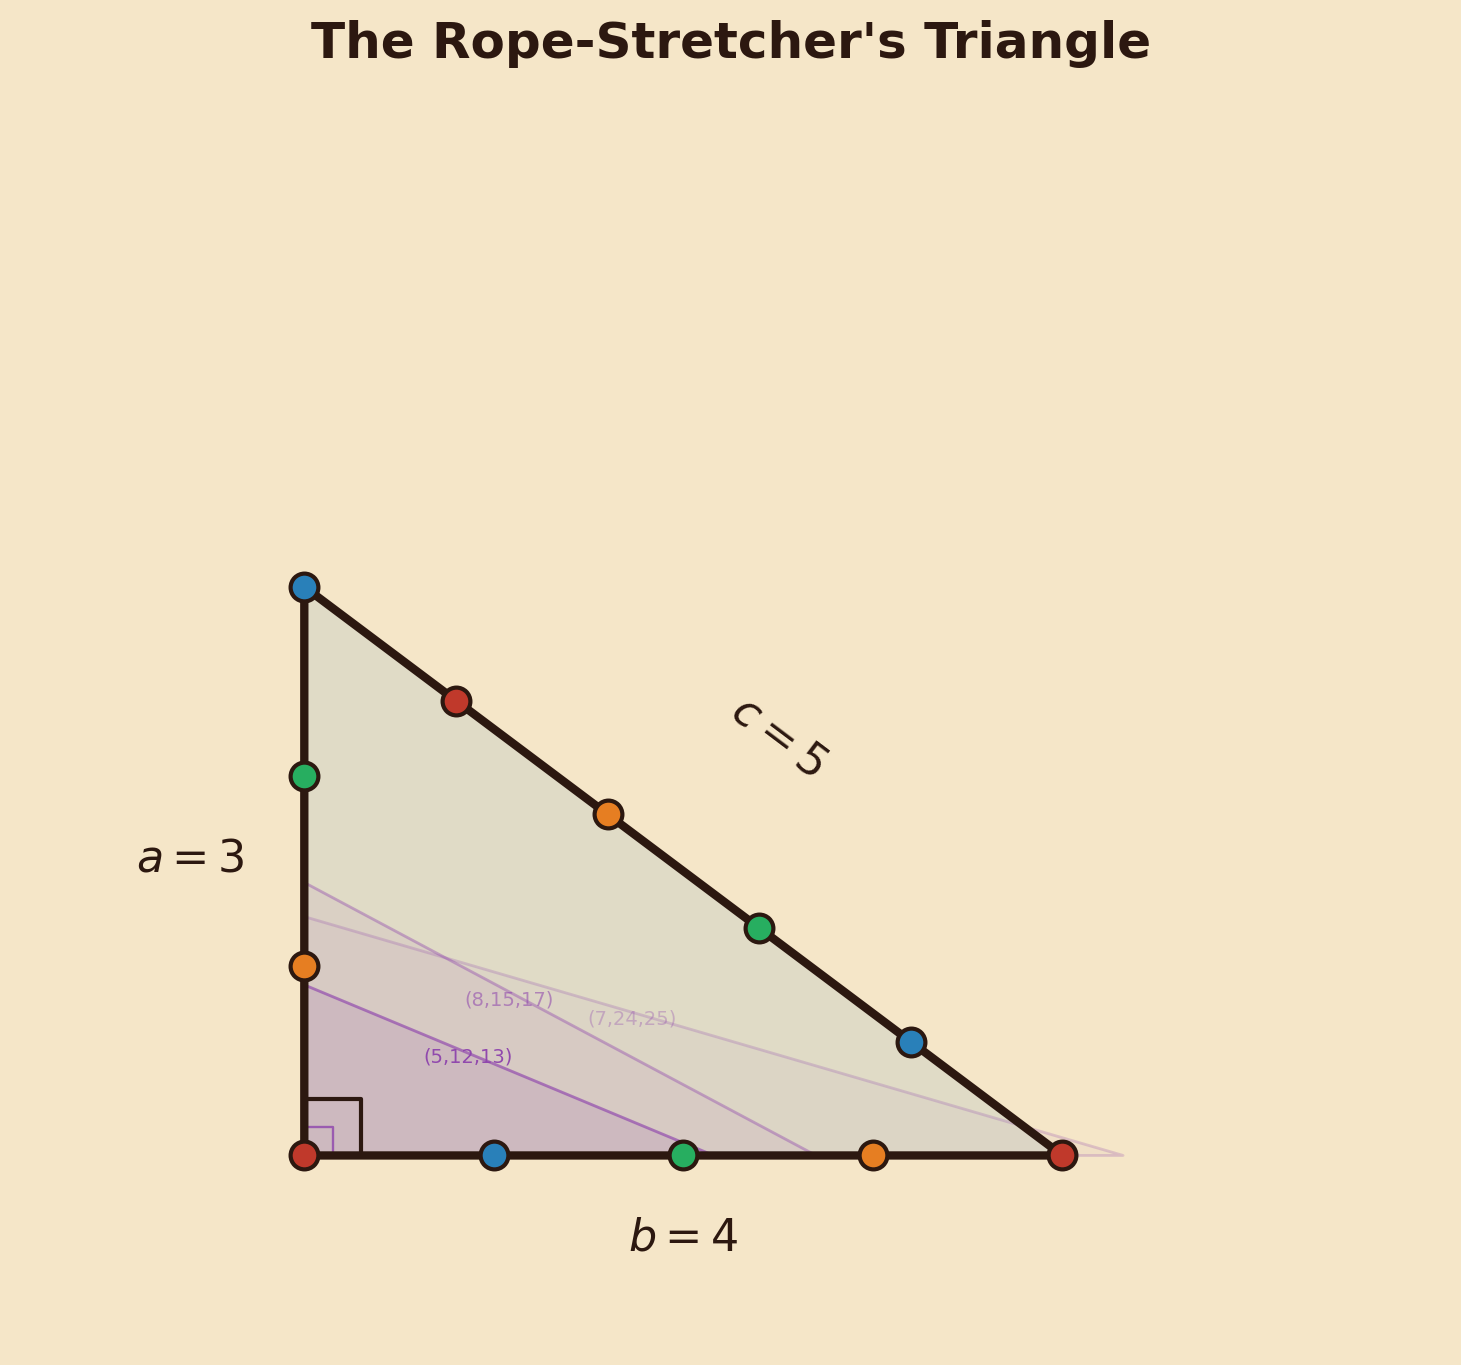
\includegraphics[width=0.75\textwidth]{../Chapter1/images/fig01_rope_triangle.png}
\caption*{Rope Triangle}
\end{figure}


\begin{figure}[htbp]
\centering
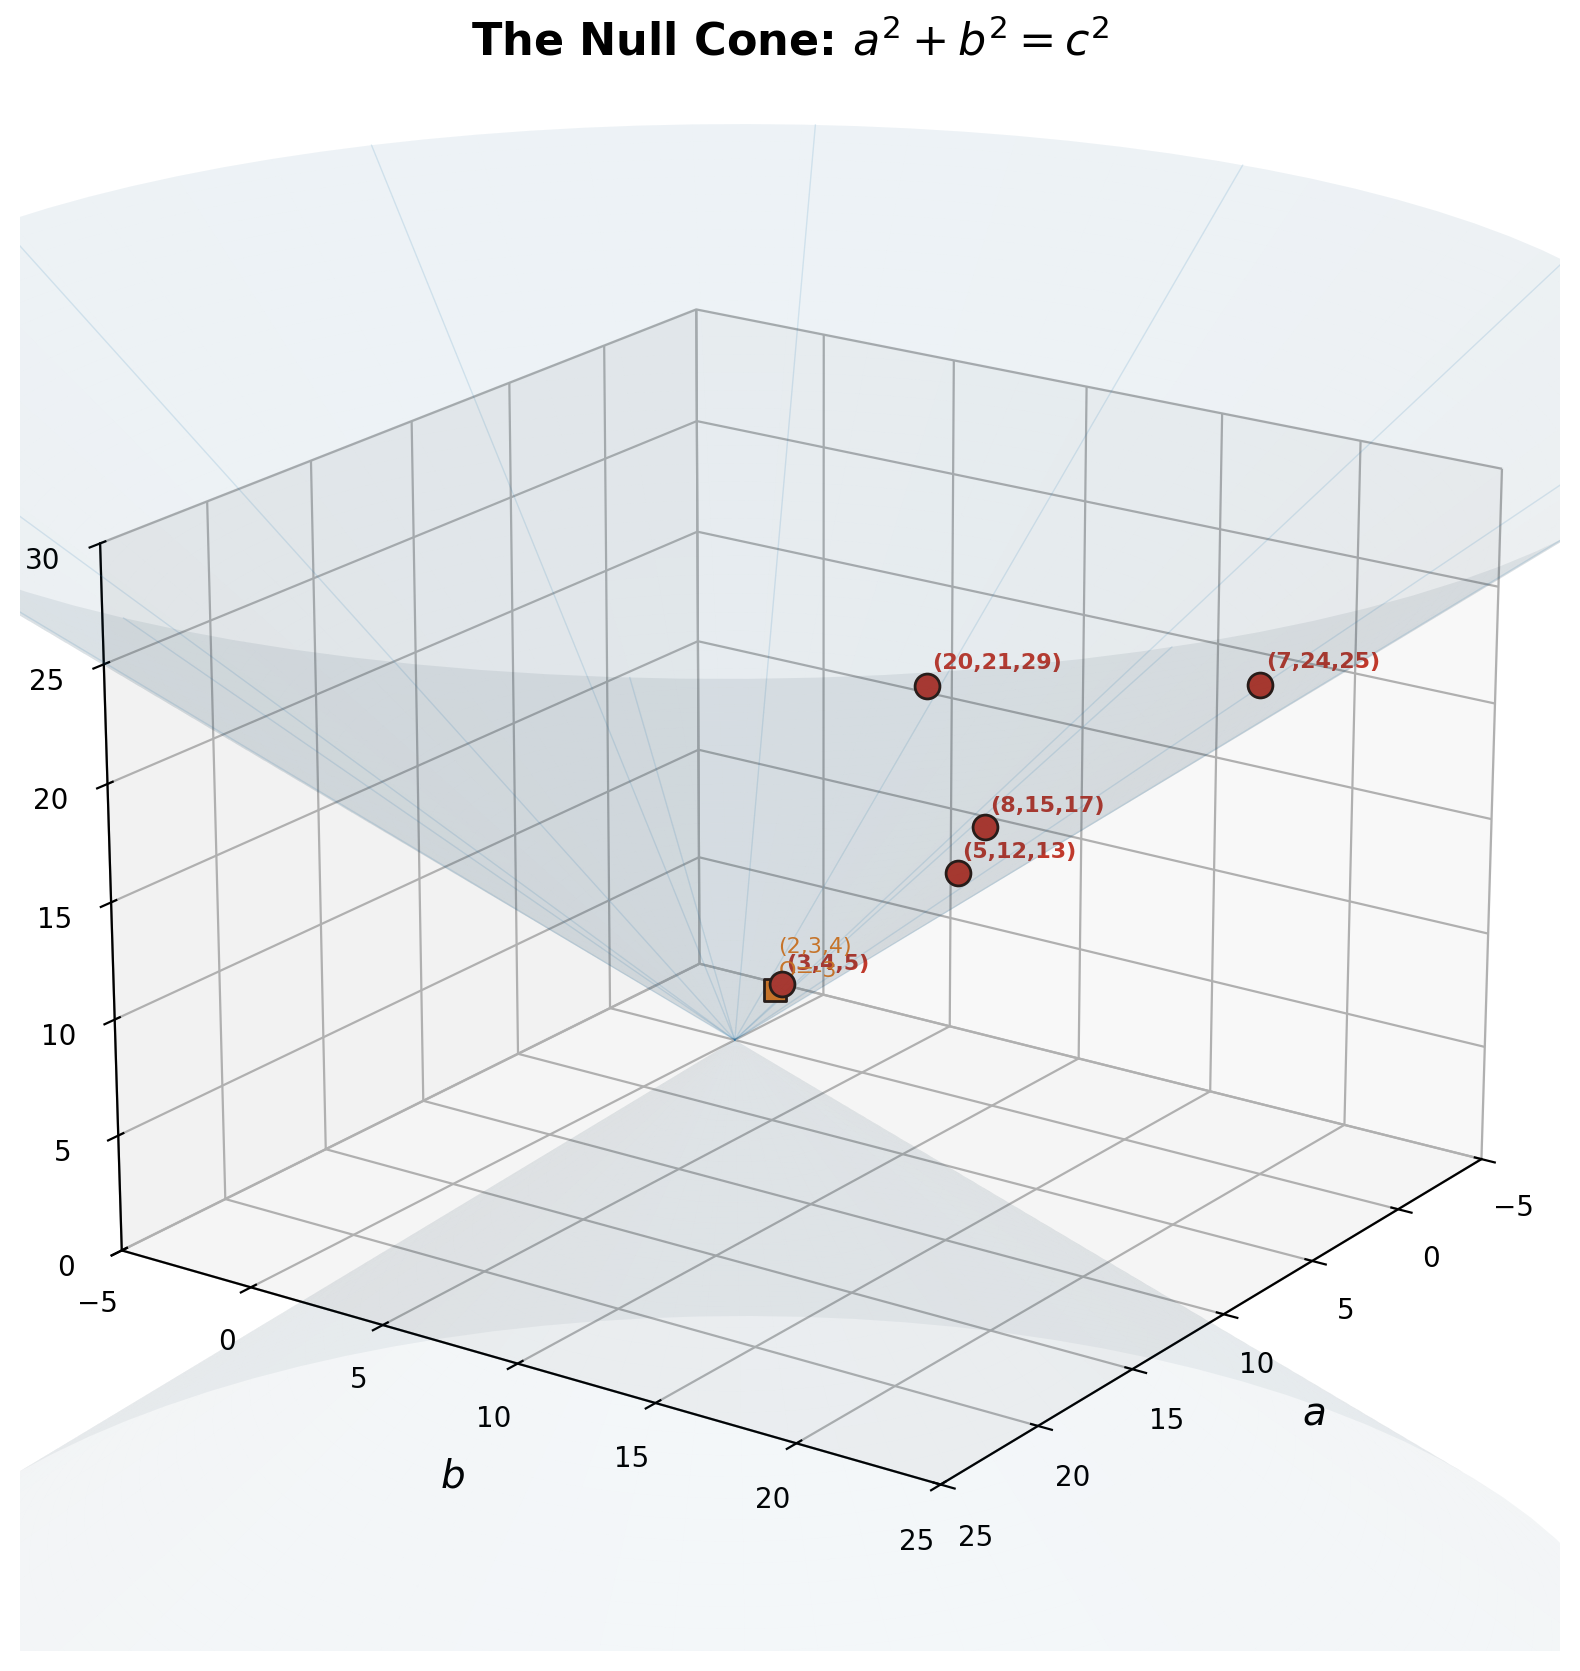
\includegraphics[width=0.75\textwidth]{../Chapter1/images/fig02_null_cone.png}
\caption*{Null Cone}
\end{figure}

\index{A Puzzle for the Pharaohs}


Imagine yourself standing on the floodplain of the Nile, somewhere around 2000 BCE. The annual inundation has just receded, leaving behind a featureless expanse of moist, black earth. Your job is to re-establish the boundaries of the barley fields --- and for that, you need right angles. No protractor. No theodolite. Just a rope.

Your forewoman hands you a length of cord with twelve equally spaced knots. She tells you to stretch it into a triangle with sides of three, four, and five knot-intervals. You plant your stakes, pull the rope taut, and --- \textit{snap} --- a perfect right angle appears at the corner between the short sides. The pharaoh's tax collectors will be satisfied; the fields are square.\index{Shor's algorithm}


The rope-stretcher's trick works because of the most famous equation in all of mathematics:

\[a^2 + b^2 = c^2.\]

Plug in $a = 3$, $b = 4$, $c = 5$: you get $9 + 16 = 25$. Perfect. A triple of positive integers $(a, b, c)$ satisfying this equation is called a \textit{Pythagorean triple}, and the ancient world was besotted with them. The Babylonians inscribed whole tables of them on clay tablets --- the celebrated Plimpton 322, dating to roughly 1800 BCE, lists at least fifteen, some with numbers in the thousands. The Egyptians stretched ropes. The Greeks elevated the subject to high art.\index{Pythagorean triple}

Here is my opening puzzle, and I invite you to set down this book and think about it before reading on:


\begin{quote}
\itshape
\textit{Is there a master list of every Pythagorean triple with no common factor --- every "primitive" one? And if so, how long is it?}
\end{quote}


The answer is breathtaking. The list is infinite --- there is no end to the right triangles with whole-number sides. Yet every single entry on it can be grown from a single seed, the humble $(3, 4, 5)$, by applying exactly three operations. The whole infinite catalogue lives in the branches of one tree. This chapter will plant that tree, watch it grow, and marvel at its fruit.

But first, a few familiar faces. Here are the primitive Pythagorean triples with hypotenuse less than 50, sorted for your convenience:\index{Pythagorean triple!primitive}


\begin{center}
\begin{tabular}{lll}
\toprule
$a$ & $b$ & $c$ \\
\midrule
3 & 4 & 5 \\
5 & 12 & 13 \\
8 & 15 & 17 \\
7 & 24 & 25 \\
20 & 21 & 29 \\
9 & 40 & 41 \\
28 & 45 & 53 \\
12 & 35 & 37 \\
11 & 60 & 61 \\
33 & 56 & 65 \\
\bottomrule
\end{tabular}
\end{center}


Stare at that table. Do you see a pattern? I wouldn't blame you if you didn't. The triples seem to pop up at random, like mushrooms after rain. There is no obvious rule, no tidy formula that predicts the next one from the last. And yet, as we shall see, every row in that table --- and every row in its infinite continuation --- hangs from the same invisible scaffold.


\bigskip\centerline{\rule{0.5\textwidth}{0.4pt}}\bigskip



\section*{The Shape of Nothing}

\begin{figure}[htbp]
\centering
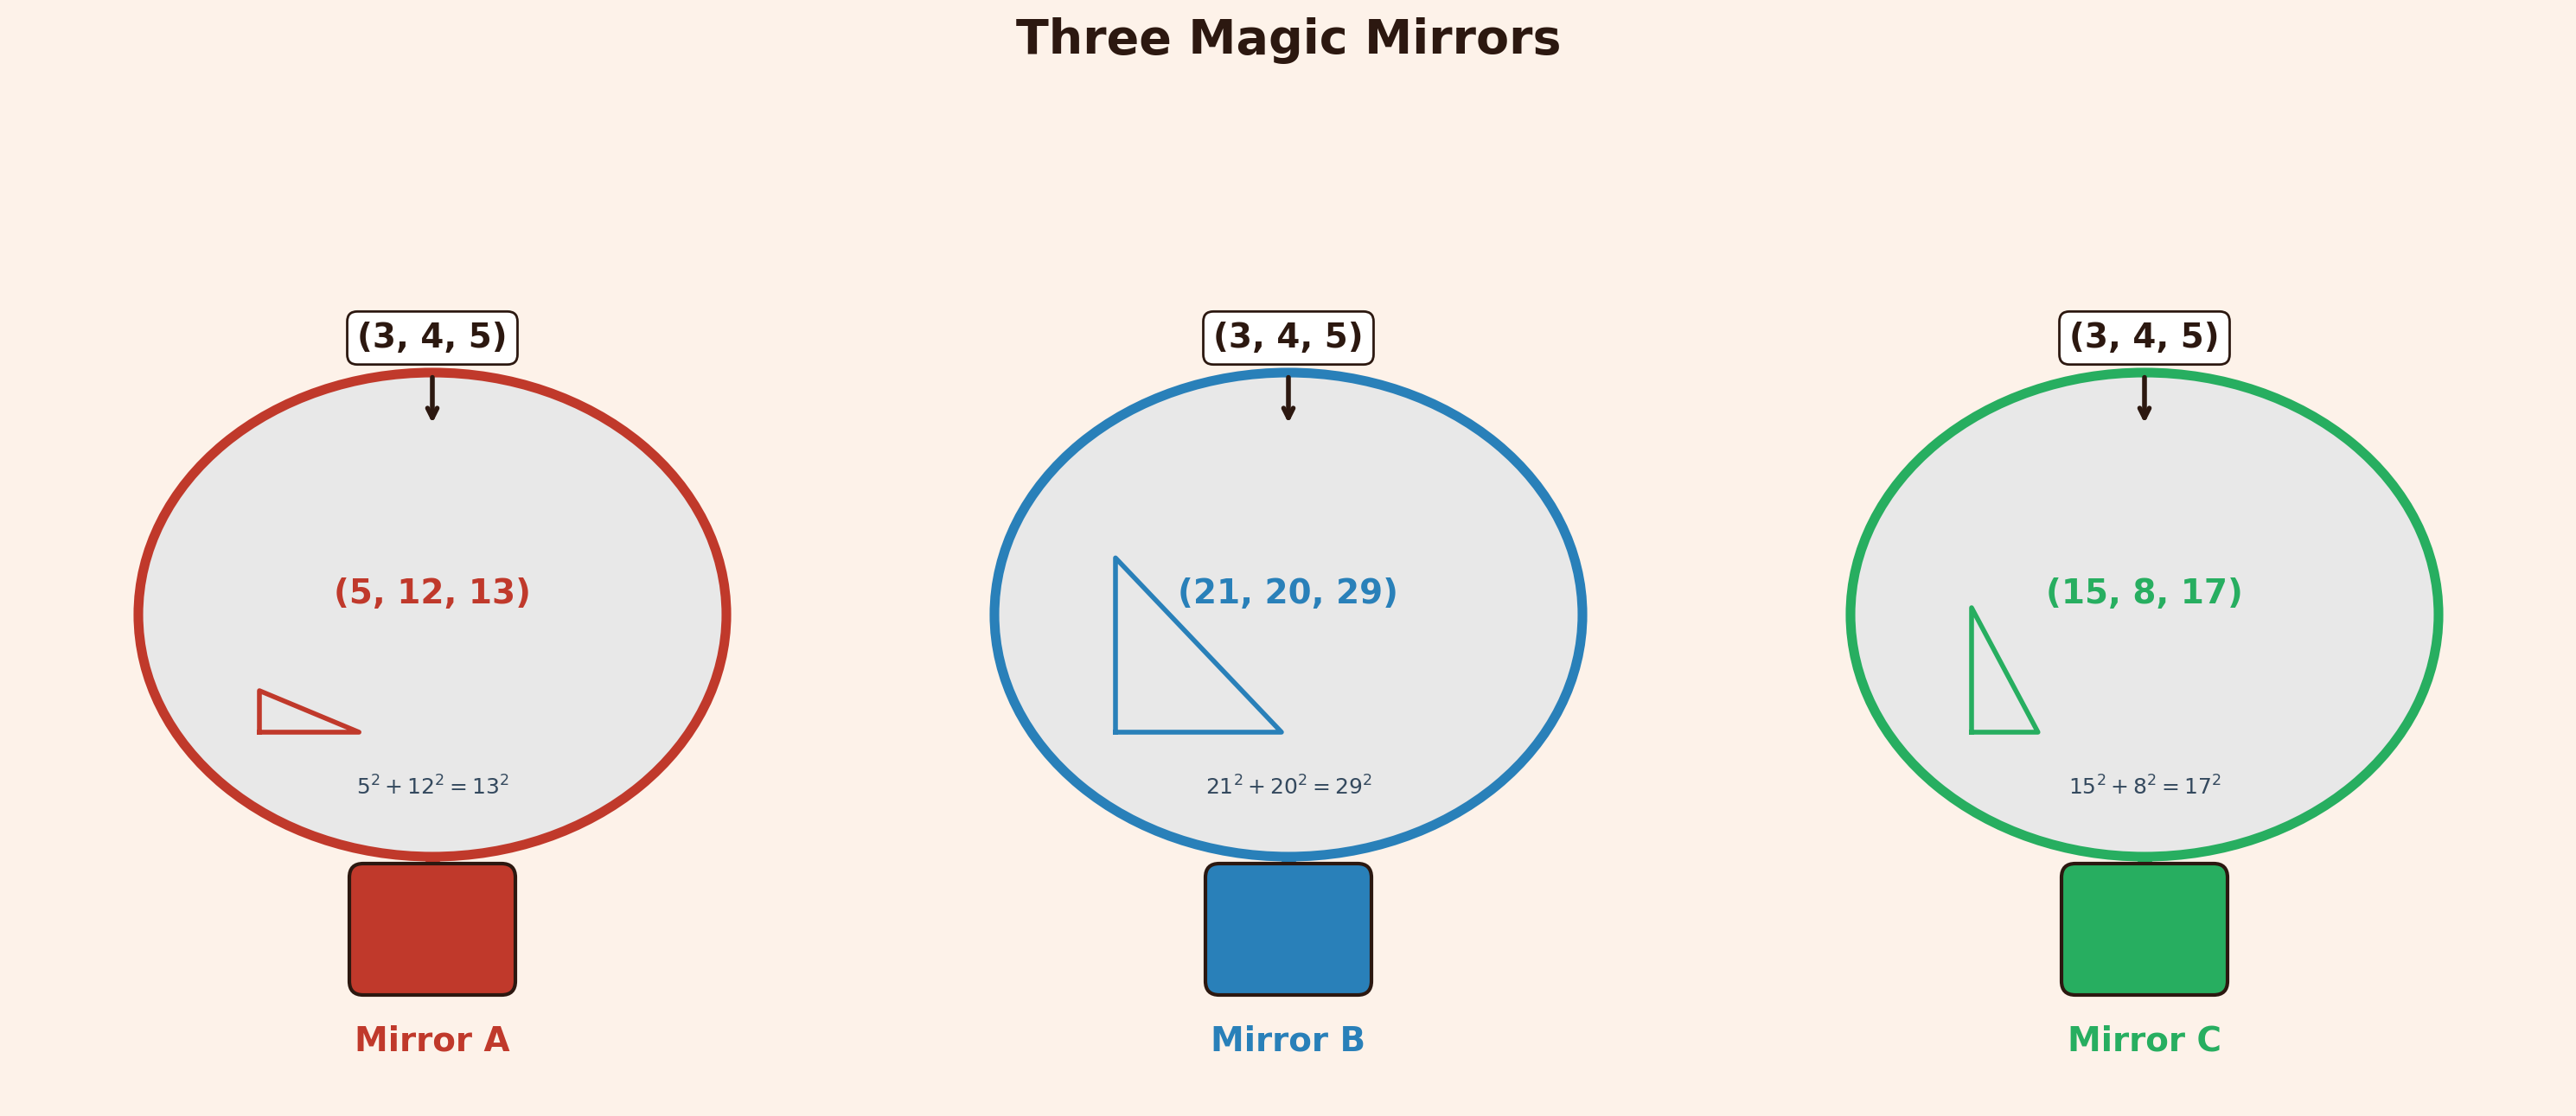
\includegraphics[width=0.75\textwidth]{../Chapter1/images/fig03_magic_mirrors.png}
\caption*{Magic Mirrors}
\end{figure}


\begin{figure}[htbp]
\centering
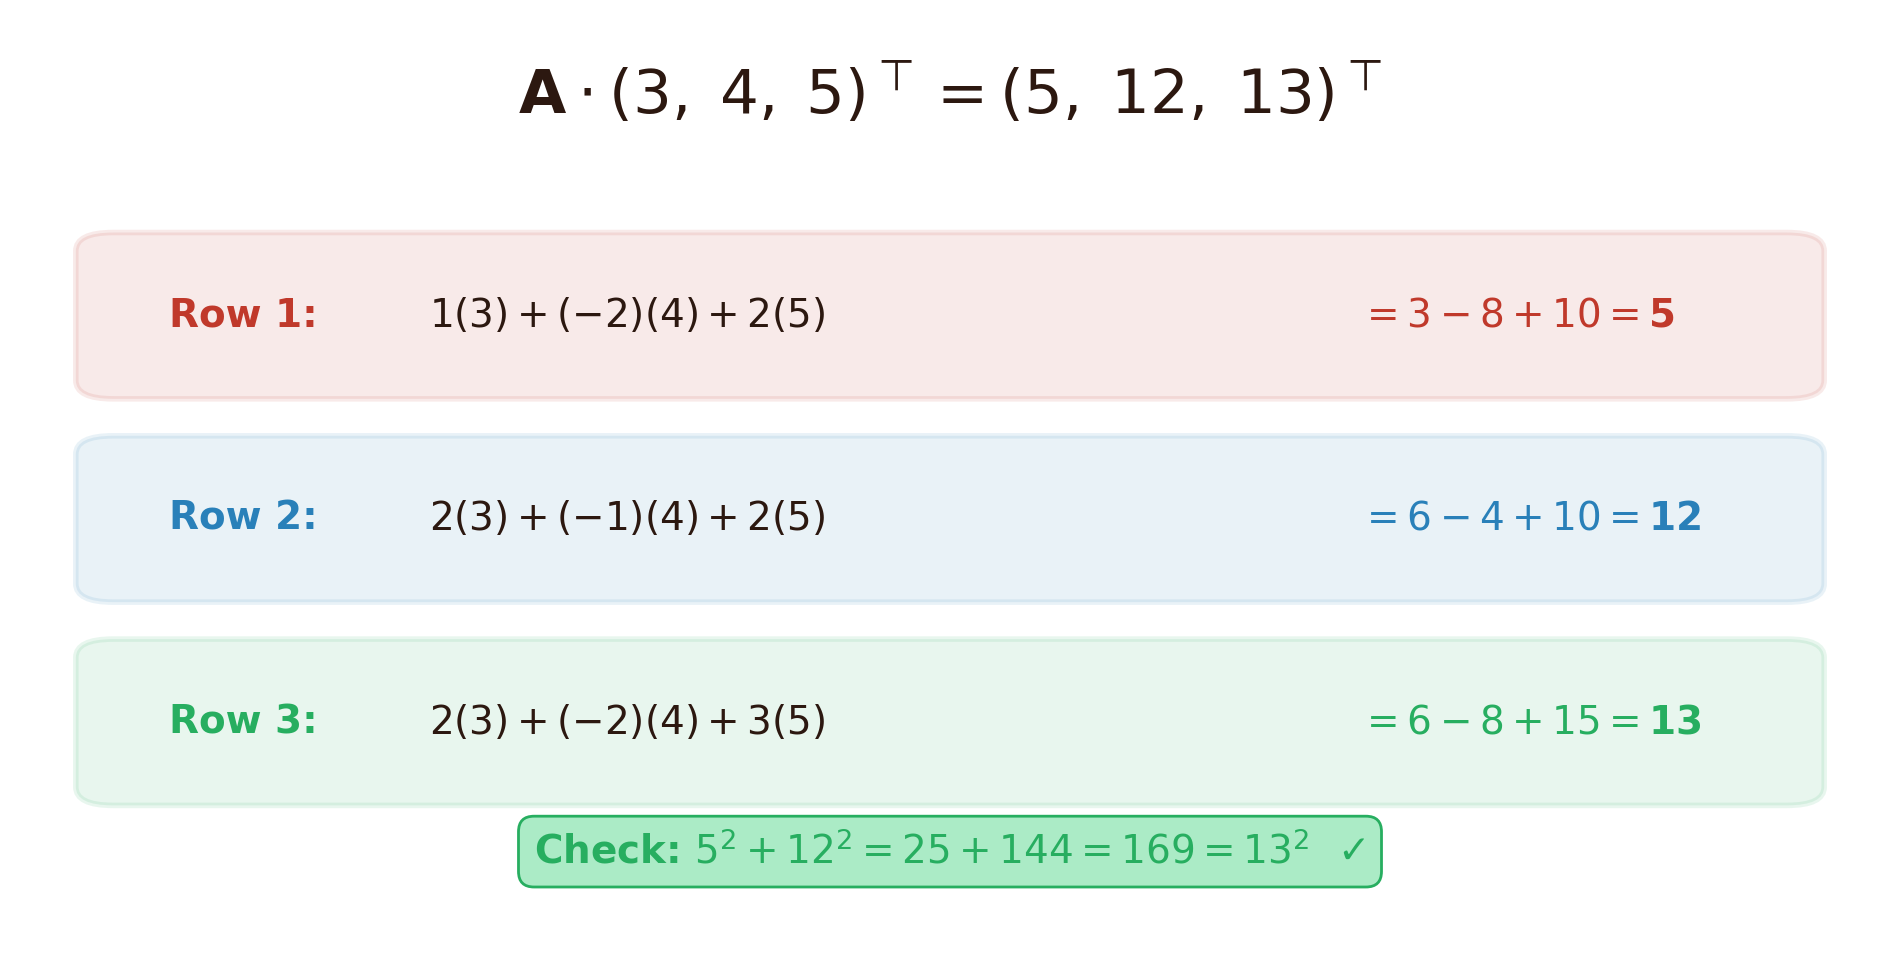
\includegraphics[width=0.75\textwidth]{../Chapter1/images/fig04_matrix_vector.png}
\caption*{Matrix Vector}
\end{figure}

\index{The Shape of Nothing}


Let us play a small game. Given any three integers $(a, b, c)$, compute

\[Q(a, b, c) = a^2 + b^2 - c^2.\]

For our old friend $(3, 4, 5)$: $Q = 9 + 16 - 25 = 0$. For $(5, 12, 13)$: $Q = 25 + 144 - 169 = 0$. Every Pythagorean triple scores \textit{zero}. That is what it \textit{means} to be Pythagorean. Now try a non-triple, say $(2, 3, 4)$: $Q = 4 + 9 - 16 = -3$. Not zero, not Pythagorean.

The function $Q$ has a name that may surprise you. Physicists call it a \textit{Lorentz quadratic form} --- the very same mathematical creature that governs the geometry of spacetime in Einstein's special relativity. In that theory, the "distance" between two events is measured not by $x^2 + y^2 + t^2$ but by $x^2 + y^2 - t^2$, with a crucial minus sign in front of the time coordinate. The surfaces where this quantity equals zero form a \textit{cone} --- the famous light cone, the boundary between the reachable future and the inaccessible elsewhere.\index{Lorentz group}


Our Pythagorean triples are exactly the \textit{integer points on the null cone} --- the lattice points where $Q$ vanishes. If we write $Q$ in matrix language,\index{null cone}

\[Q(\mathbf{v}) = \mathbf{v}^\top \mathbf{Q}\, \mathbf{v}, \qquad \mathbf{Q} = \begin{pmatrix} 1 & 0 & 0 \\ 0 & 1 & 0 \\ 0 & 0 & -1 \end{pmatrix}, \qquad \mathbf{v} = \begin{pmatrix} a \\ b \\ c \end{pmatrix},\]

then the Pythagorean equation is simply $\mathbf{v}^\top \mathbf{Q}\, \mathbf{v} = 0$. The ancient Babylonians and Albert Einstein were, unknowingly, studying the same equation. One sought right triangles for surveying; the other sought the invariants of the universe. Mathematics, as usual, does not care about your motivation.\index{Einstein, Albert}


\bigskip\centerline{\rule{0.5\textwidth}{0.4pt}}\bigskip



\section*{Three Magic Mirrors}

\begin{figure}[htbp]
\centering
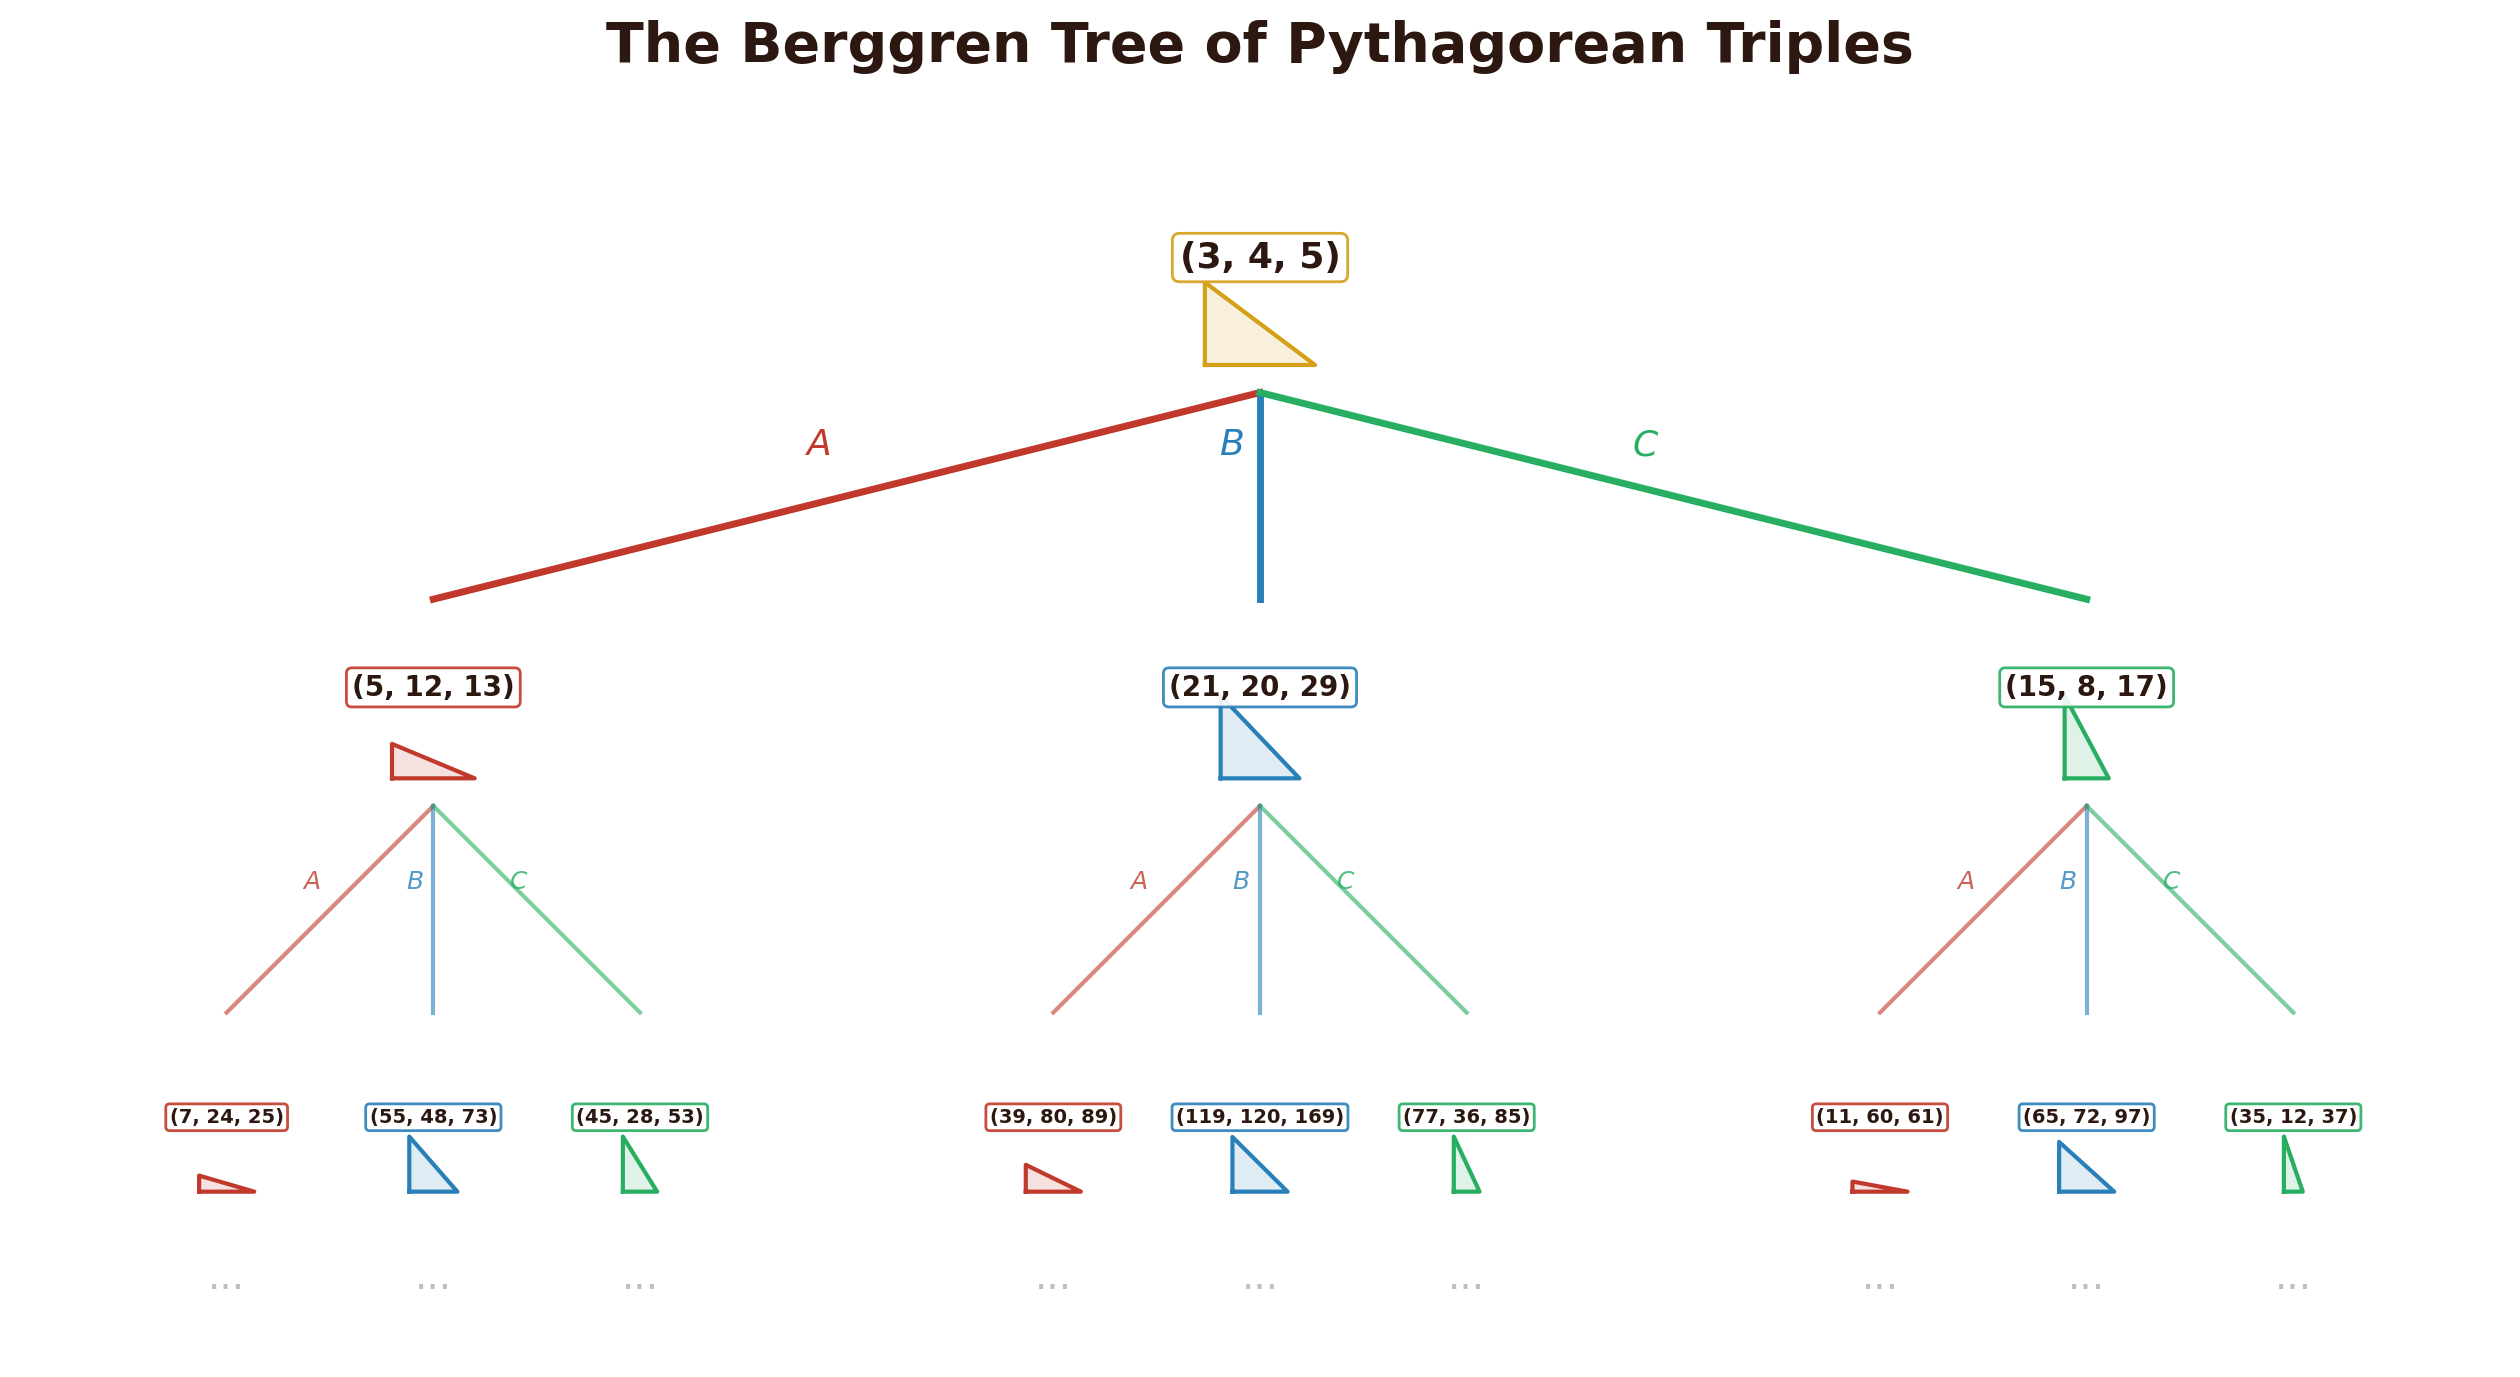
\includegraphics[width=0.75\textwidth]{../Chapter1/images/fig05_berggren_tree.png}
\caption*{Berggren Tree}
\end{figure}


\begin{figure}[htbp]
\centering
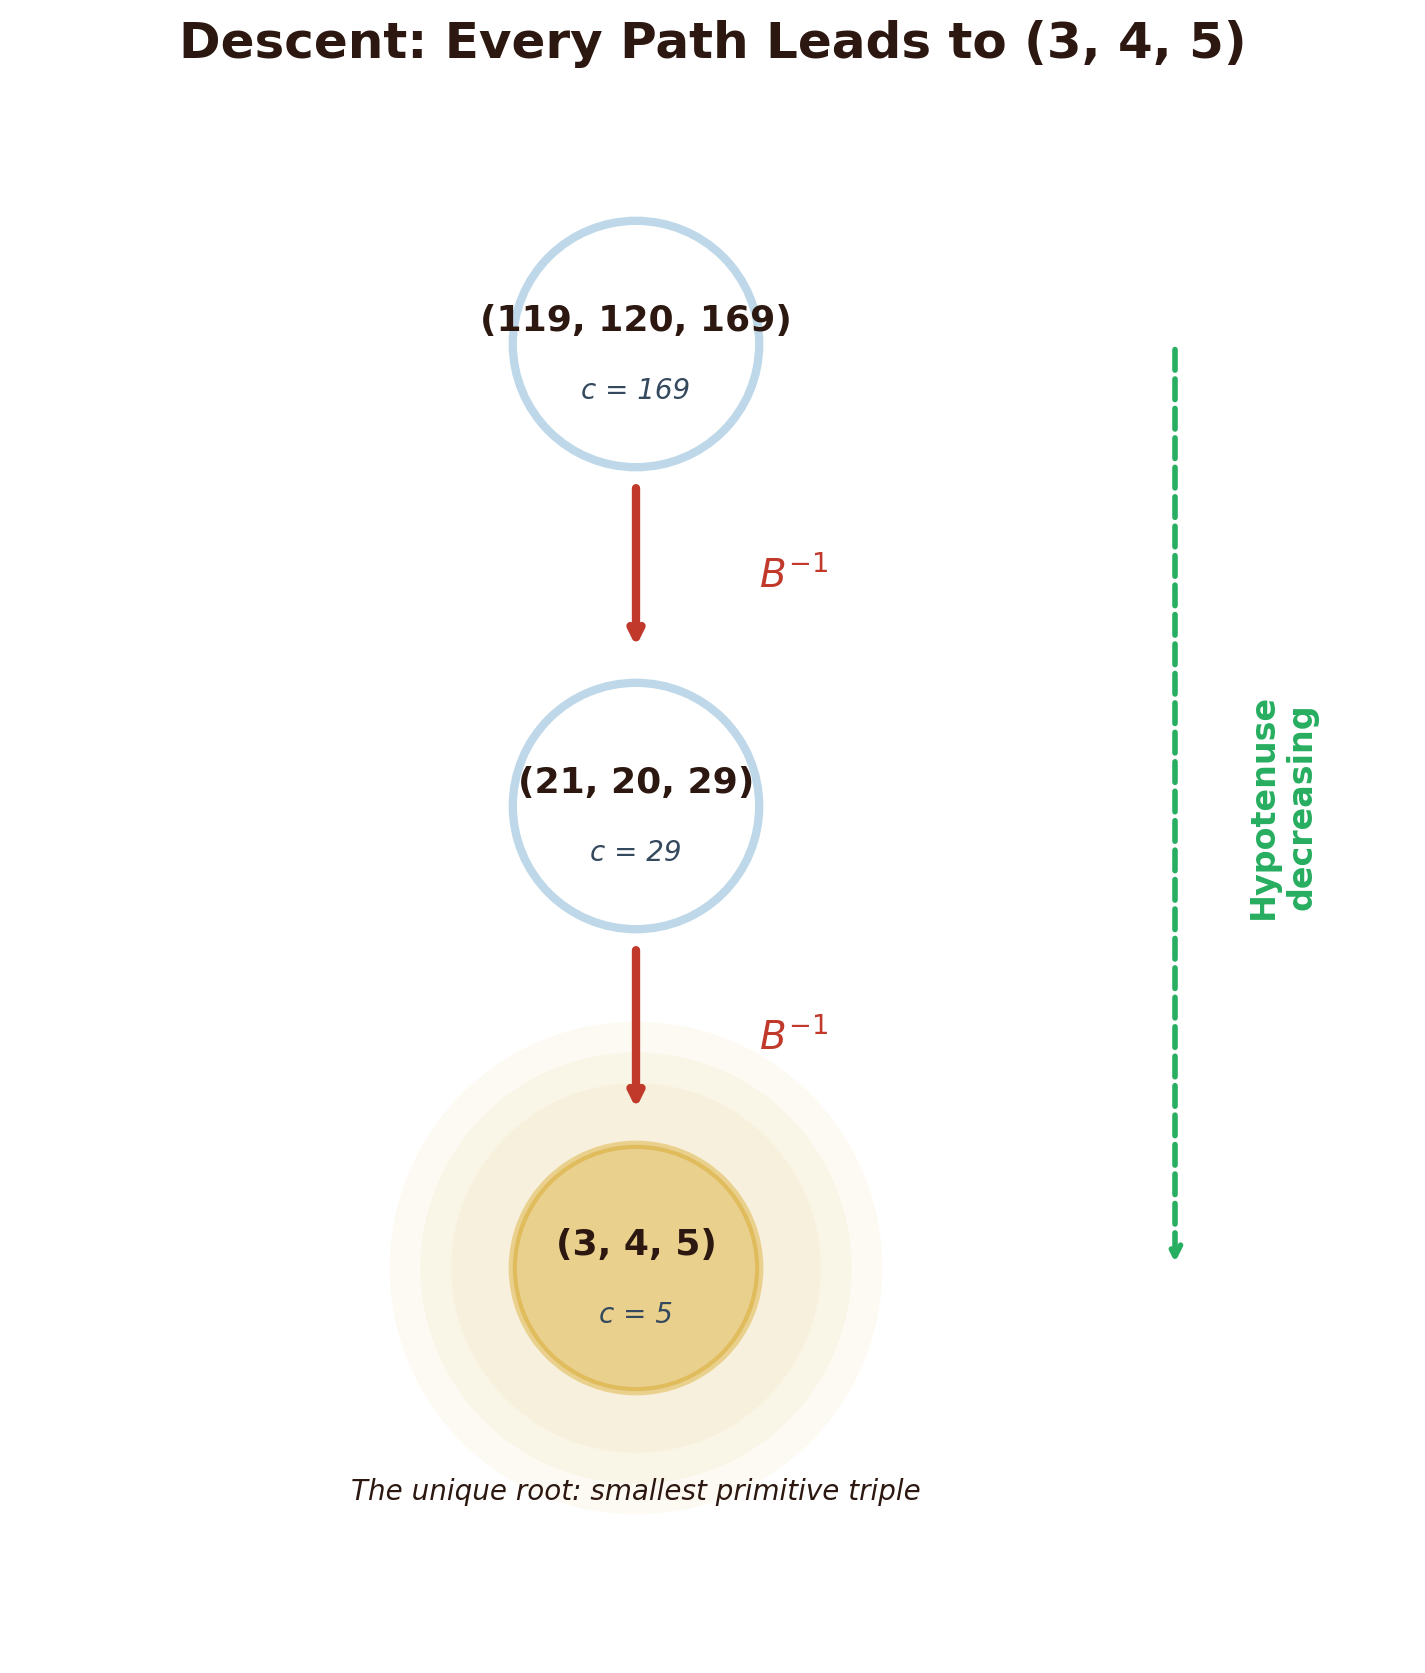
\includegraphics[width=0.75\textwidth]{../Chapter1/images/fig06_descent_maze.png}
\caption*{Descent Maze}
\end{figure}

\index{Three Magic Mirrors}


Now comes the card trick. Write $(3, 4, 5)$ on a card. I will hand you three "magic mirrors" --- matrices labeled $\mathbf{A}$, $\mathbf{B}$, and $\mathbf{C}$ --- and each one will transform your triple into a \textit{new} Pythagorean triple:

\[\mathbf{A}: (3, 4, 5) \;\longmapsto\; (5, 12, 13)\]
\[\mathbf{B}: (3, 4, 5) \;\longmapsto\; (21, 20, 29)\]
\[\mathbf{C}: (3, 4, 5) \;\longmapsto\; (15, 8, 17)\]

Go ahead --- verify each one. $5^2 + 12^2 = 25 + 144 = 169 = 13^2$. Check. $21^2 + 20^2 = 441 + 400 = 841 = 29^2$. Check. $15^2 + 8^2 = 225 + 64 = 289 = 17^2$. Check. The trick never fails. \textit{Why?}

Here are the mirrors:

\[\mathbf{A} = \begin{pmatrix} 1 & -2 & 2 \\ 2 & -1 & 2 \\ 2 & -2 & 3 \end{pmatrix}, \quad
\mathbf{B} = \begin{pmatrix} 1 & 2 & 2 \\ 2 & 1 & 2 \\ 2 & 2 & 3 \end{pmatrix}, \quad
\mathbf{C} = \begin{pmatrix} -1 & 2 & 2 \\ -2 & 1 & 2 \\ -2 & 2 & 3 \end{pmatrix}\]


Each matrix was discovered by the Swedish mathematician Berggren in a remarkable 1934 paper that was almost entirely forgotten until it was independently rediscovered by Barning in 1963 and Hall in 1970. Such is the sociology of mathematics: a result can be proven, published, and ignored for three decades, only to spring back to life when the world is finally ready for it.

The reason the trick works is both simple and profound. Each matrix $\mathbf{M}$ satisfies the identity

\[\mathbf{M}^\top \mathbf{Q}\, \mathbf{M} = \mathbf{Q}.\]

In plain language: the mirror preserves the Lorentz form. If $Q(\mathbf{v}) = 0$ --- if the input lies on the null cone --- then $Q(\mathbf{M}\mathbf{v}) = \mathbf{v}^\top \mathbf{M}^\top \mathbf{Q}\, \mathbf{M}\, \mathbf{v} = \mathbf{v}^\top \mathbf{Q}\, \mathbf{v} = 0$. The output lies on the cone too. \textit{The mirrors preserve the shape of nothing.}

Let us verify this for $\mathbf{A}$ the honest way, by expanding everything. If $(a, b, c)$ is Pythagorean, define the new triple as

\[a' = a - 2b + 2c, \quad b' = 2a - b + 2c, \quad c' = 2a - 2b + 3c.\]

Now compute $a'^2 + b'^2 - c'^2$ by brute force --- expand each square, collect terms, and watch the cross-terms annihilate each other until all that remains is $a^2 + b^2 - c^2$. The algebra is a wonderful exercise for a rainy afternoon, and I encourage every reader to carry it out at least once. It is pure magic performed in slow motion: dozens of terms appear, dance in pairs, and vanish, leaving behind exactly the expression you started with. Zero in, zero out.



\bigskip\centerline{\rule{0.5\textwidth}{0.4pt}}\bigskip



\section*{An Infinite Family Tree}

\begin{figure}[htbp]
\centering
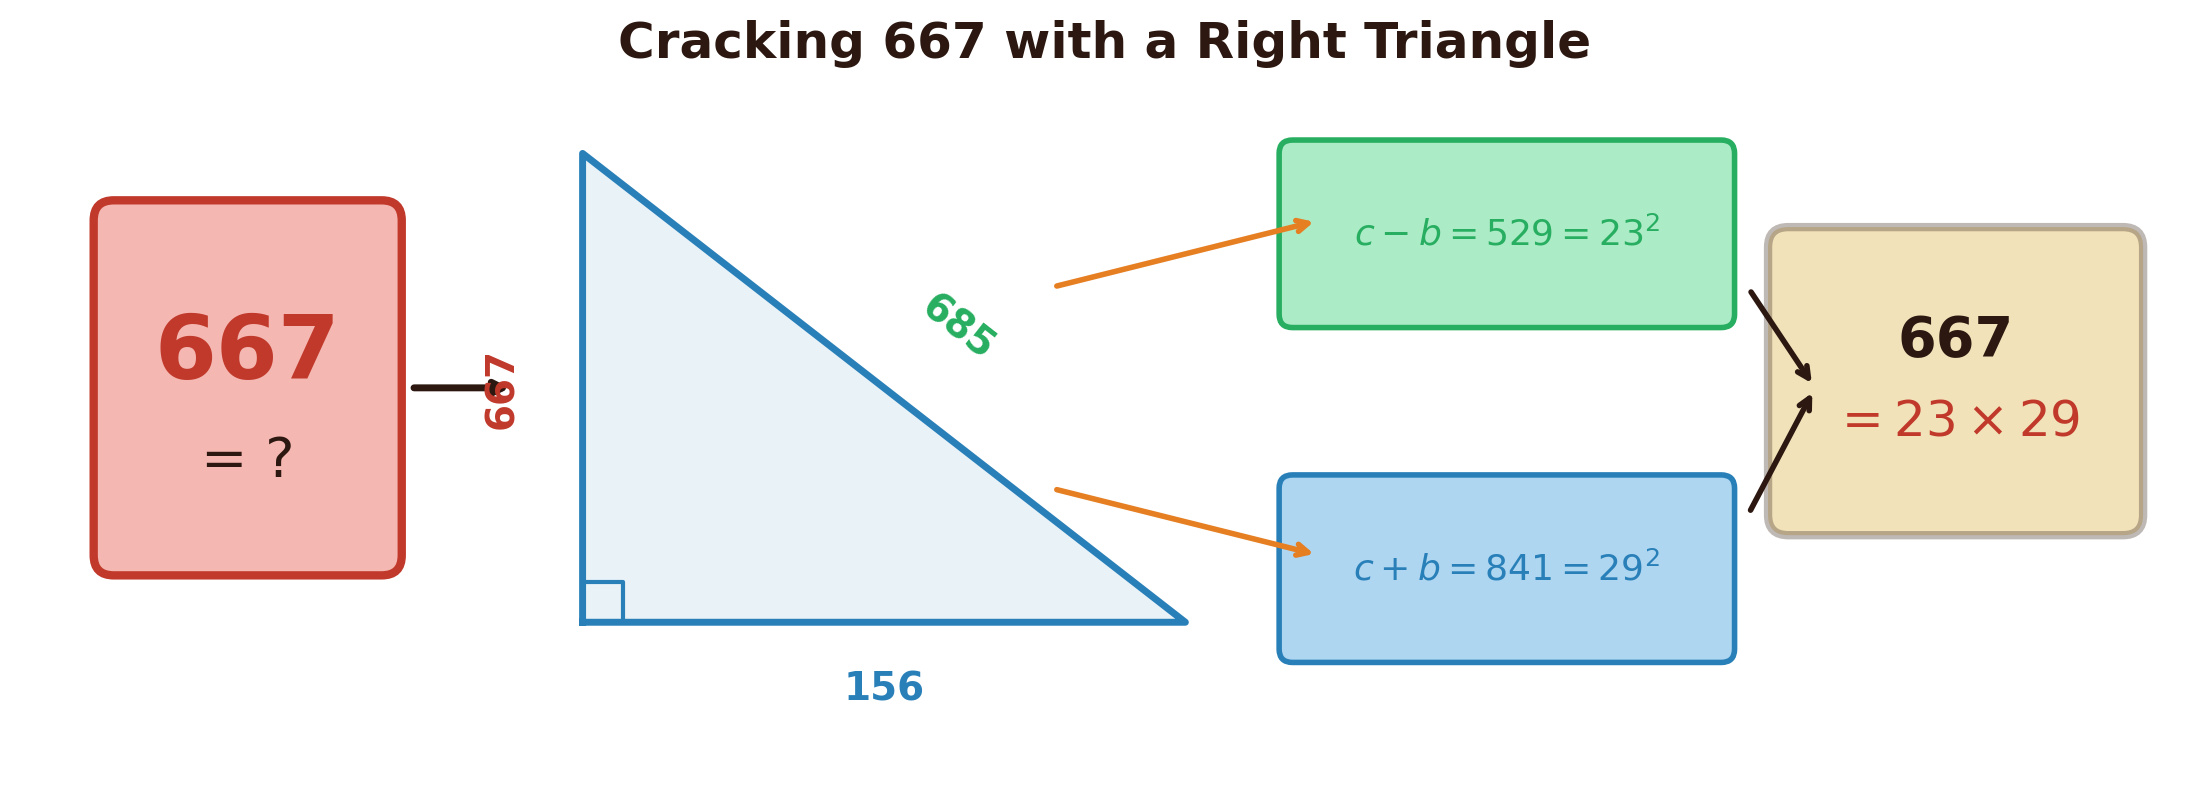
\includegraphics[width=0.75\textwidth]{../Chapter1/images/fig07_factoring_trick.png}
\caption*{Factoring Trick}
\end{figure}


\begin{figure}[htbp]
\centering
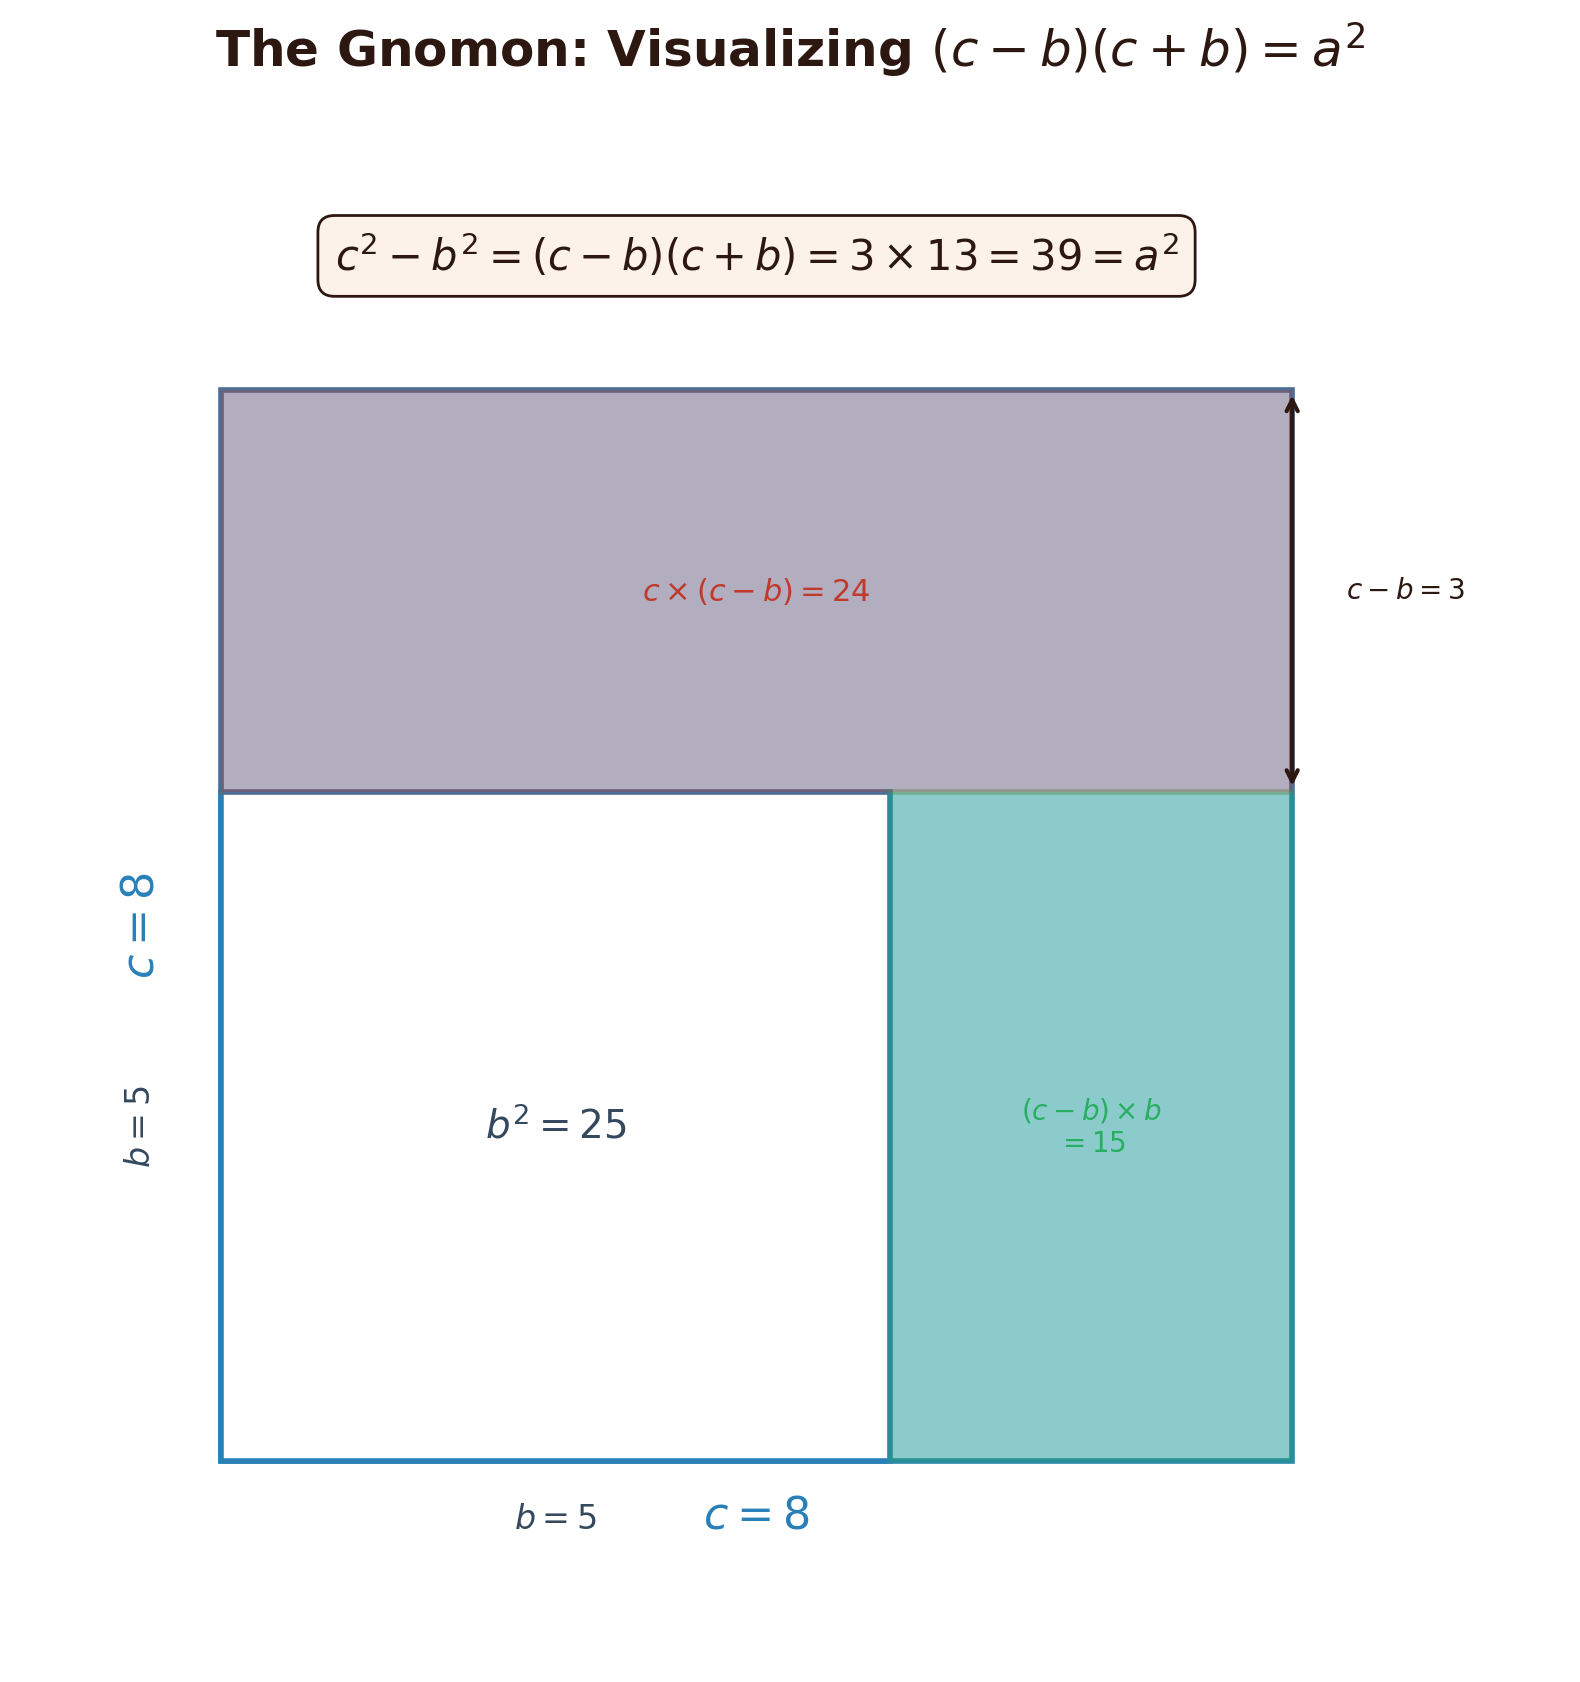
\includegraphics[width=0.75\textwidth]{../Chapter1/images/fig08_gnomon.png}
\caption*{Gnomon}
\end{figure}

\index{An Infinite Family Tree}


Every human being on Earth has exactly one mother and one father. But what if every \textit{right triangle} had exactly three children --- and a single common ancestor?

That is precisely the structure of the \textbf{Berggren tree}. It is a rooted ternary tree with $(3, 4, 5)$ at the root. Each node $(a, b, c)$ has three children, obtained by applying $\mathbf{A}$, $\mathbf{B}$, and $\mathbf{C}$:\index{Berggren tree}

\[
(3,4,5) \xrightarrow{\;\mathbf{A}\;} (5,12,13), \qquad
(3,4,5) \xrightarrow{\;\mathbf{B}\;} (21,20,29), \qquad
(3,4,5) \xrightarrow{\;\mathbf{C}\;} (15,8,17).\]

Each of those children spawns three children of its own:

\[
(5,12,13) \xrightarrow{\;\mathbf{A}\;} (7,24,25), \qquad
(5,12,13) \xrightarrow{\;\mathbf{B}\;} (55,48,73), \qquad
(5,12,13) \xrightarrow{\;\mathbf{C}\;} (45,28,53).\]

And so on, forever. The tree never terminates, never repeats, and --- here is the grand theorem that will occupy us for much of this book --- \textit{never misses a single primitive Pythagorean triple}. Every primitive triple appears exactly once, at a unique address in the tree. The tree is a complete, irredundant catalogue.


The \textit{depth} of a triple is the number of matrix applications needed to reach it from the root: $(3,4,5)$ has depth $0$; its three children have depth $1$; the nine grandchildren have depth $2$. At depth $d$, there are $3^d$ triples --- three at depth $1$, nine at depth $2$, twenty-seven at depth $3$, and so on. The tree is a portrait of infinity, branching relentlessly into the number line.


\bigskip\centerline{\rule{0.5\textwidth}{0.4pt}}\bigskip



\section*{Climbing Down the Tree}

\begin{figure}[htbp]
\centering
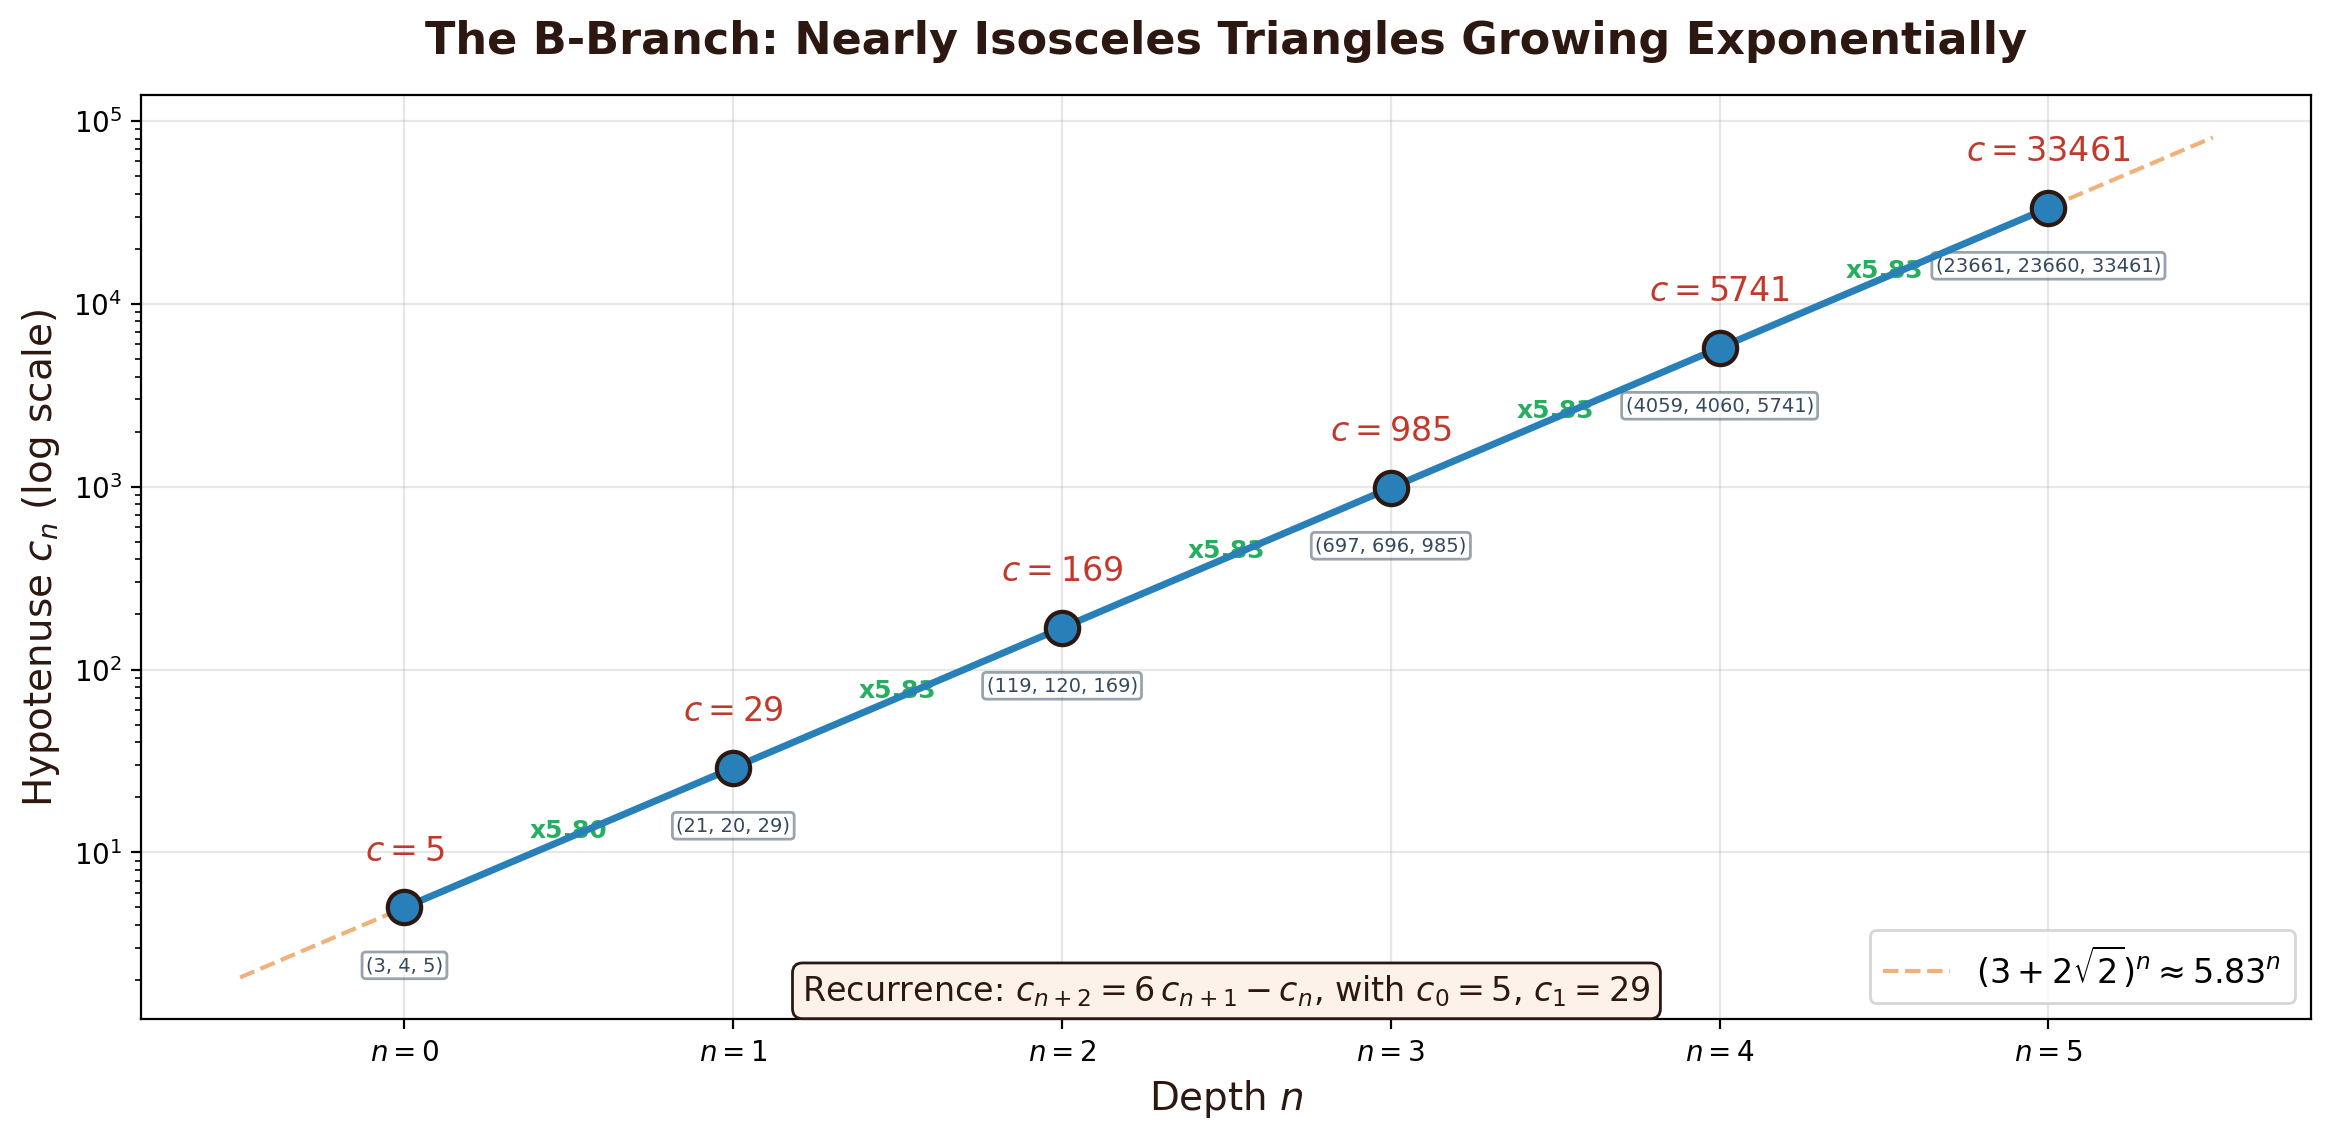
\includegraphics[width=0.75\textwidth]{../Chapter1/images/fig09_b_branch.png}
\caption*{B Branch}
\end{figure}


\begin{figure}[htbp]
\centering
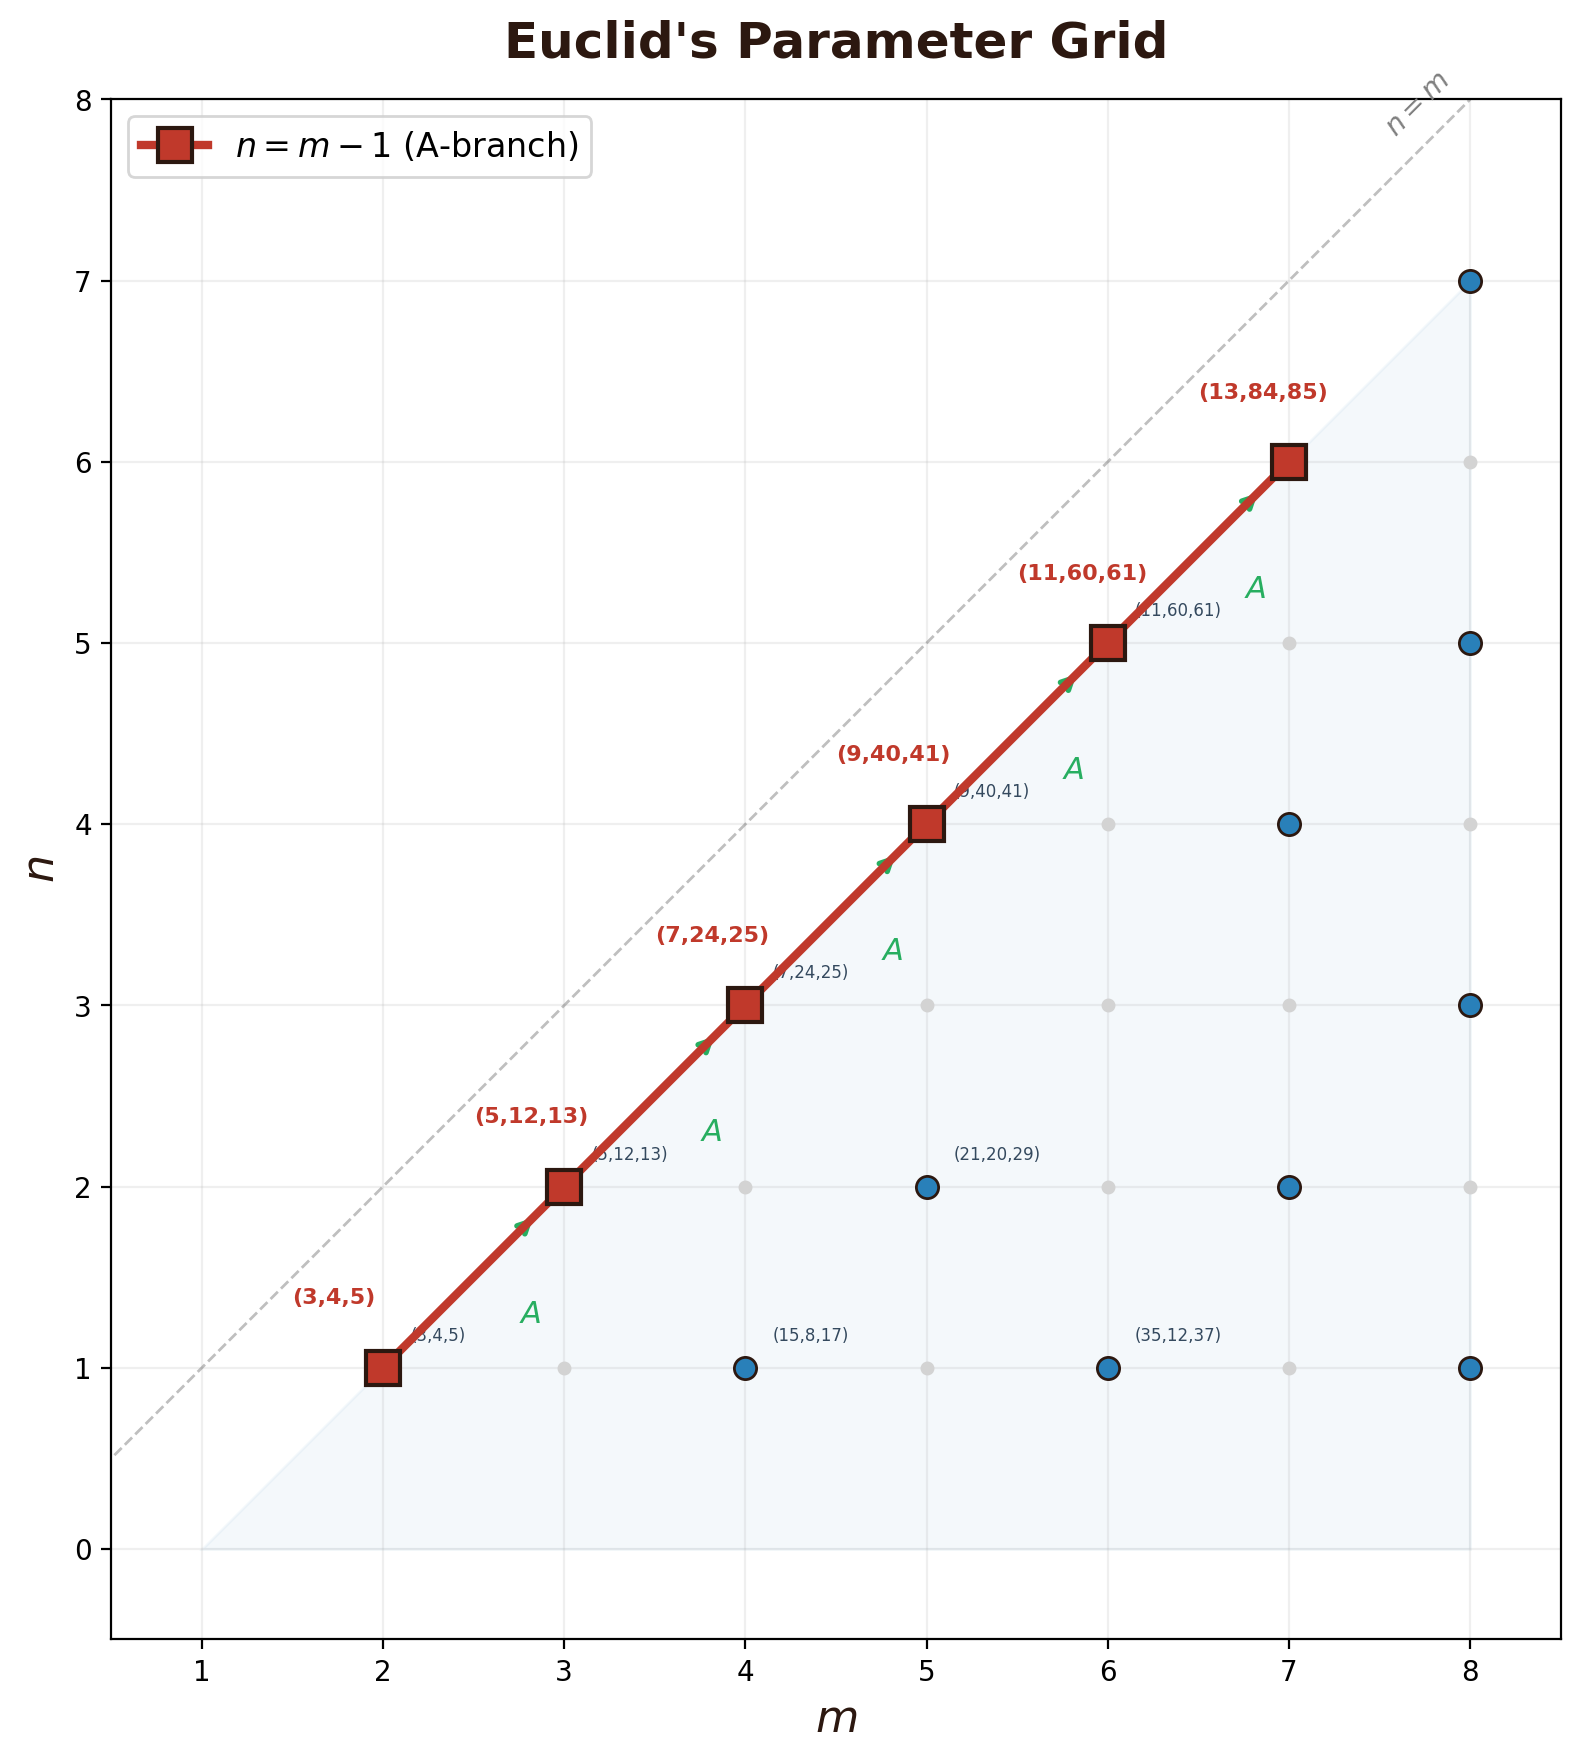
\includegraphics[width=0.75\textwidth]{../Chapter1/images/fig10_euclid_grid.png}
\caption*{Euclid Grid}
\end{figure}

\index{Climbing Down the Tree}


Suppose I hand you a Pythagorean triple with a hypotenuse of ten million. Can you trace it \textit{backward} through the tree to $(3, 4, 5)$? And more importantly, are you guaranteed to arrive there, or might you wander forever?

The answer is yes, you are guaranteed, and the reason is beautiful. Each of the three matrices has an inverse --- a matrix that undoes its transformation. The determinants are $\det(\mathbf{A}) = 1$, $\det(\mathbf{B}) = -1$, $\det(\mathbf{C}) = 1$ --- all $\pm 1$ --- so the inverses are also integer matrices. (A matrix with integer entries and determinant $\pm 1$ always has an integer inverse. This is one of those facts that sounds like it should be hard to prove, but it follows immediately from the formula for the inverse in terms of cofactors.)

Now here is the key insight. For any primitive triple with $c > 5$, applying the correct inverse matrix produces a new triple whose hypotenuse is \textit{strictly smaller}. The proof is disarmingly simple:

\[(a + b)^2 = a^2 + 2ab + b^2 > a^2 + b^2 = c^2,\]

so $a + b > c$. Therefore $2(a + b) > 2c$, which gives us $3c - 2a - 2b < c$. Since the hypotenuse is a positive integer that strictly decreases at each step, the descent must terminate --- and the only place it \textit{can} terminate is at $(3, 4, 5)$, the unique primitive triple with the smallest hypotenuse.\index{descent}


This is a descent argument --- a technique with a glorious pedigree stretching back to Fermat himself, who used "infinite descent" to prove that $x^4 + y^4 = z^2$ has no positive integer solutions. The idea is always the same: if a counterexample existed, you could construct a smaller one, then a smaller one still, then a smaller one again… but positive integers cannot decrease forever. Contradiction.\index{Fermat, Pierre de}


\bigskip\centerline{\rule{0.5\textwidth}{0.4pt}}\bigskip



\section*{Cracking Numbers with Triangles}

\begin{figure}[htbp]
\centering
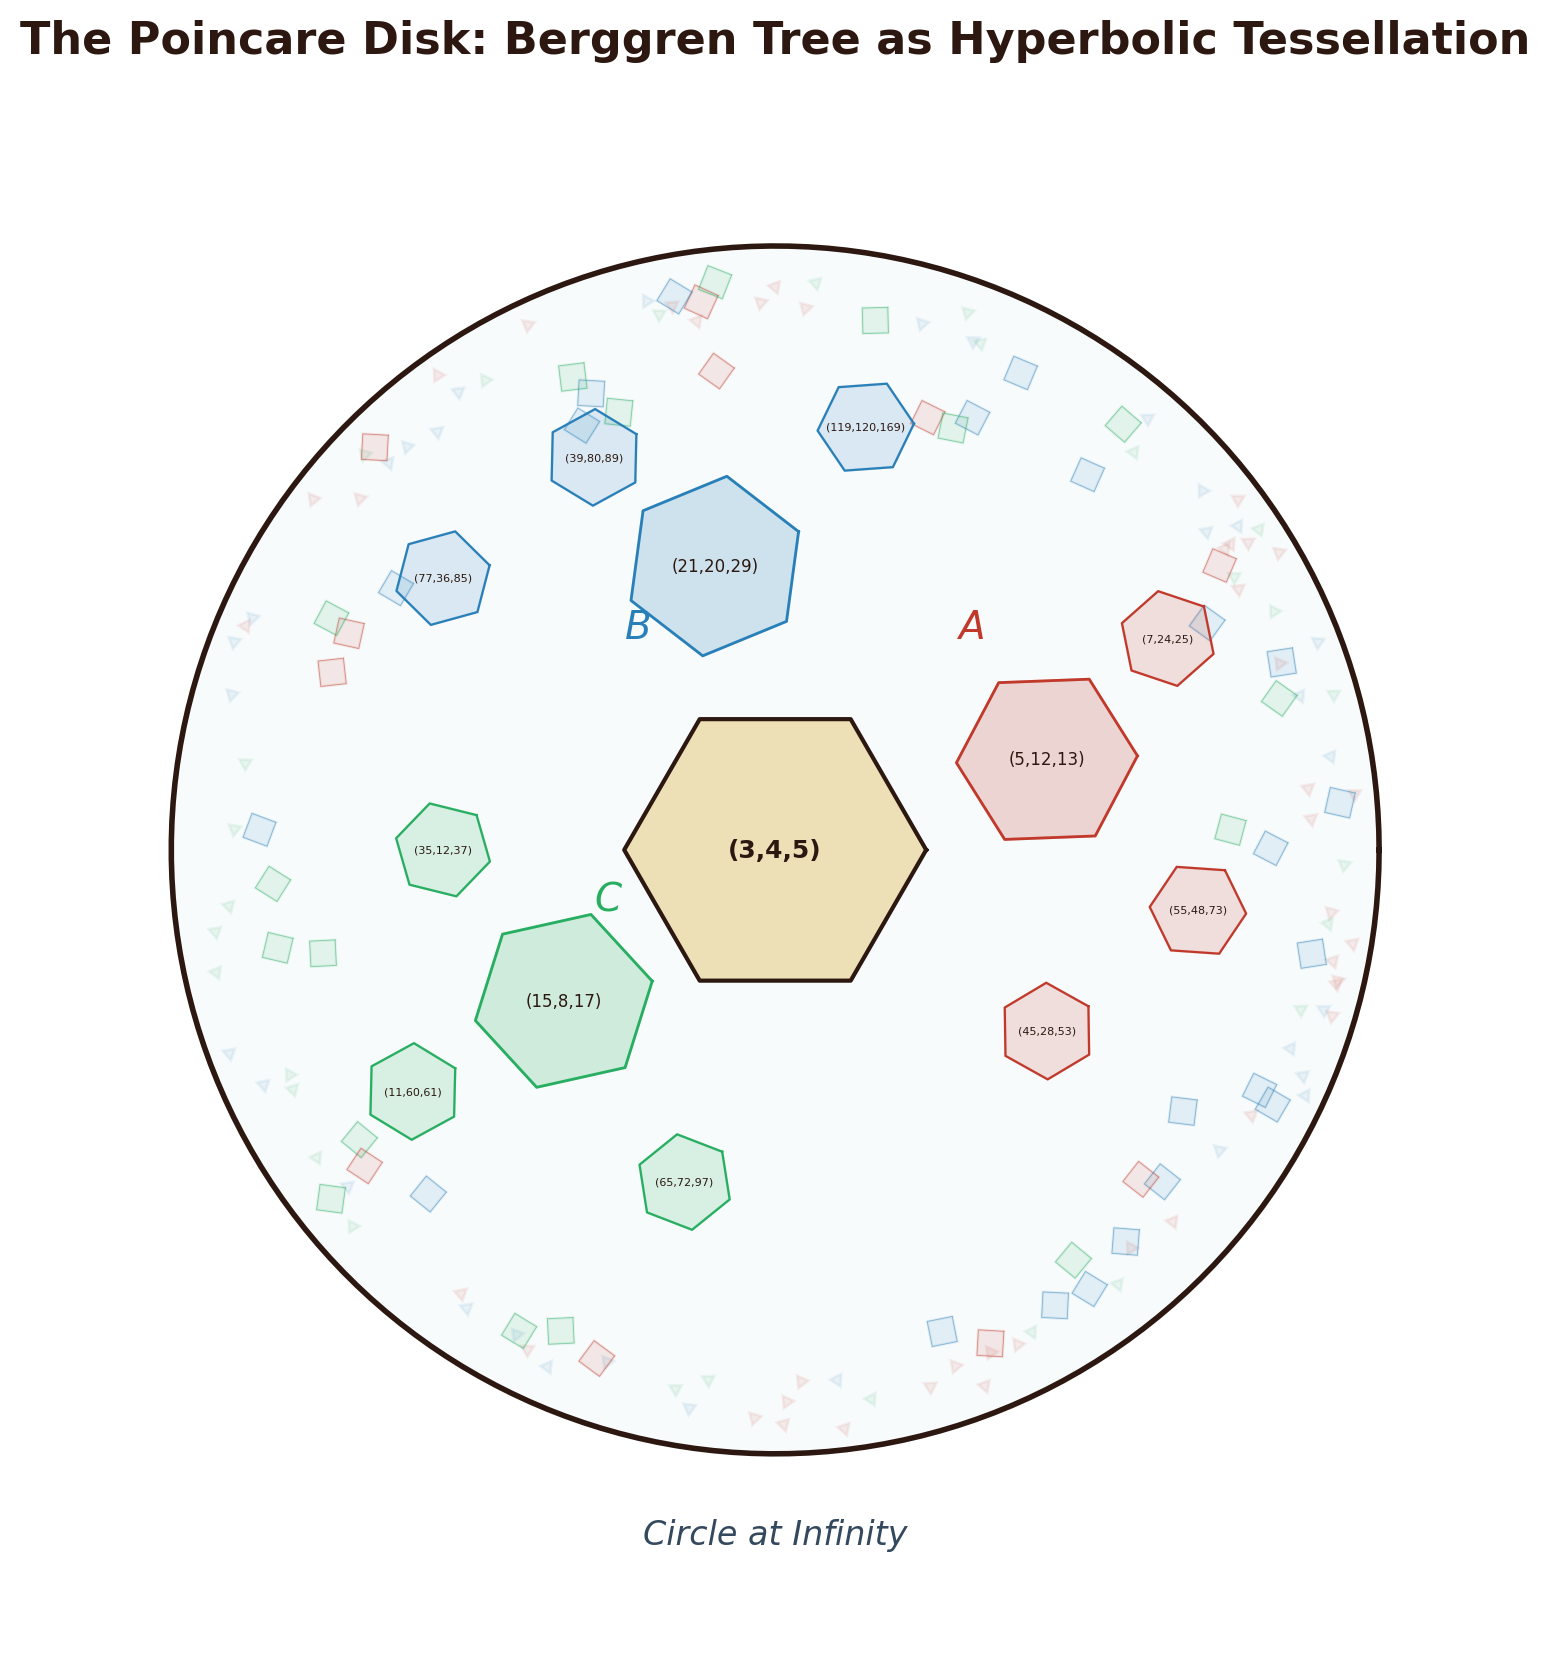
\includegraphics[width=0.75\textwidth]{../Chapter1/images/fig11_poincare_disk.png}
\caption*{Poincare Disk}
\end{figure}


\begin{figure}[htbp]
\centering
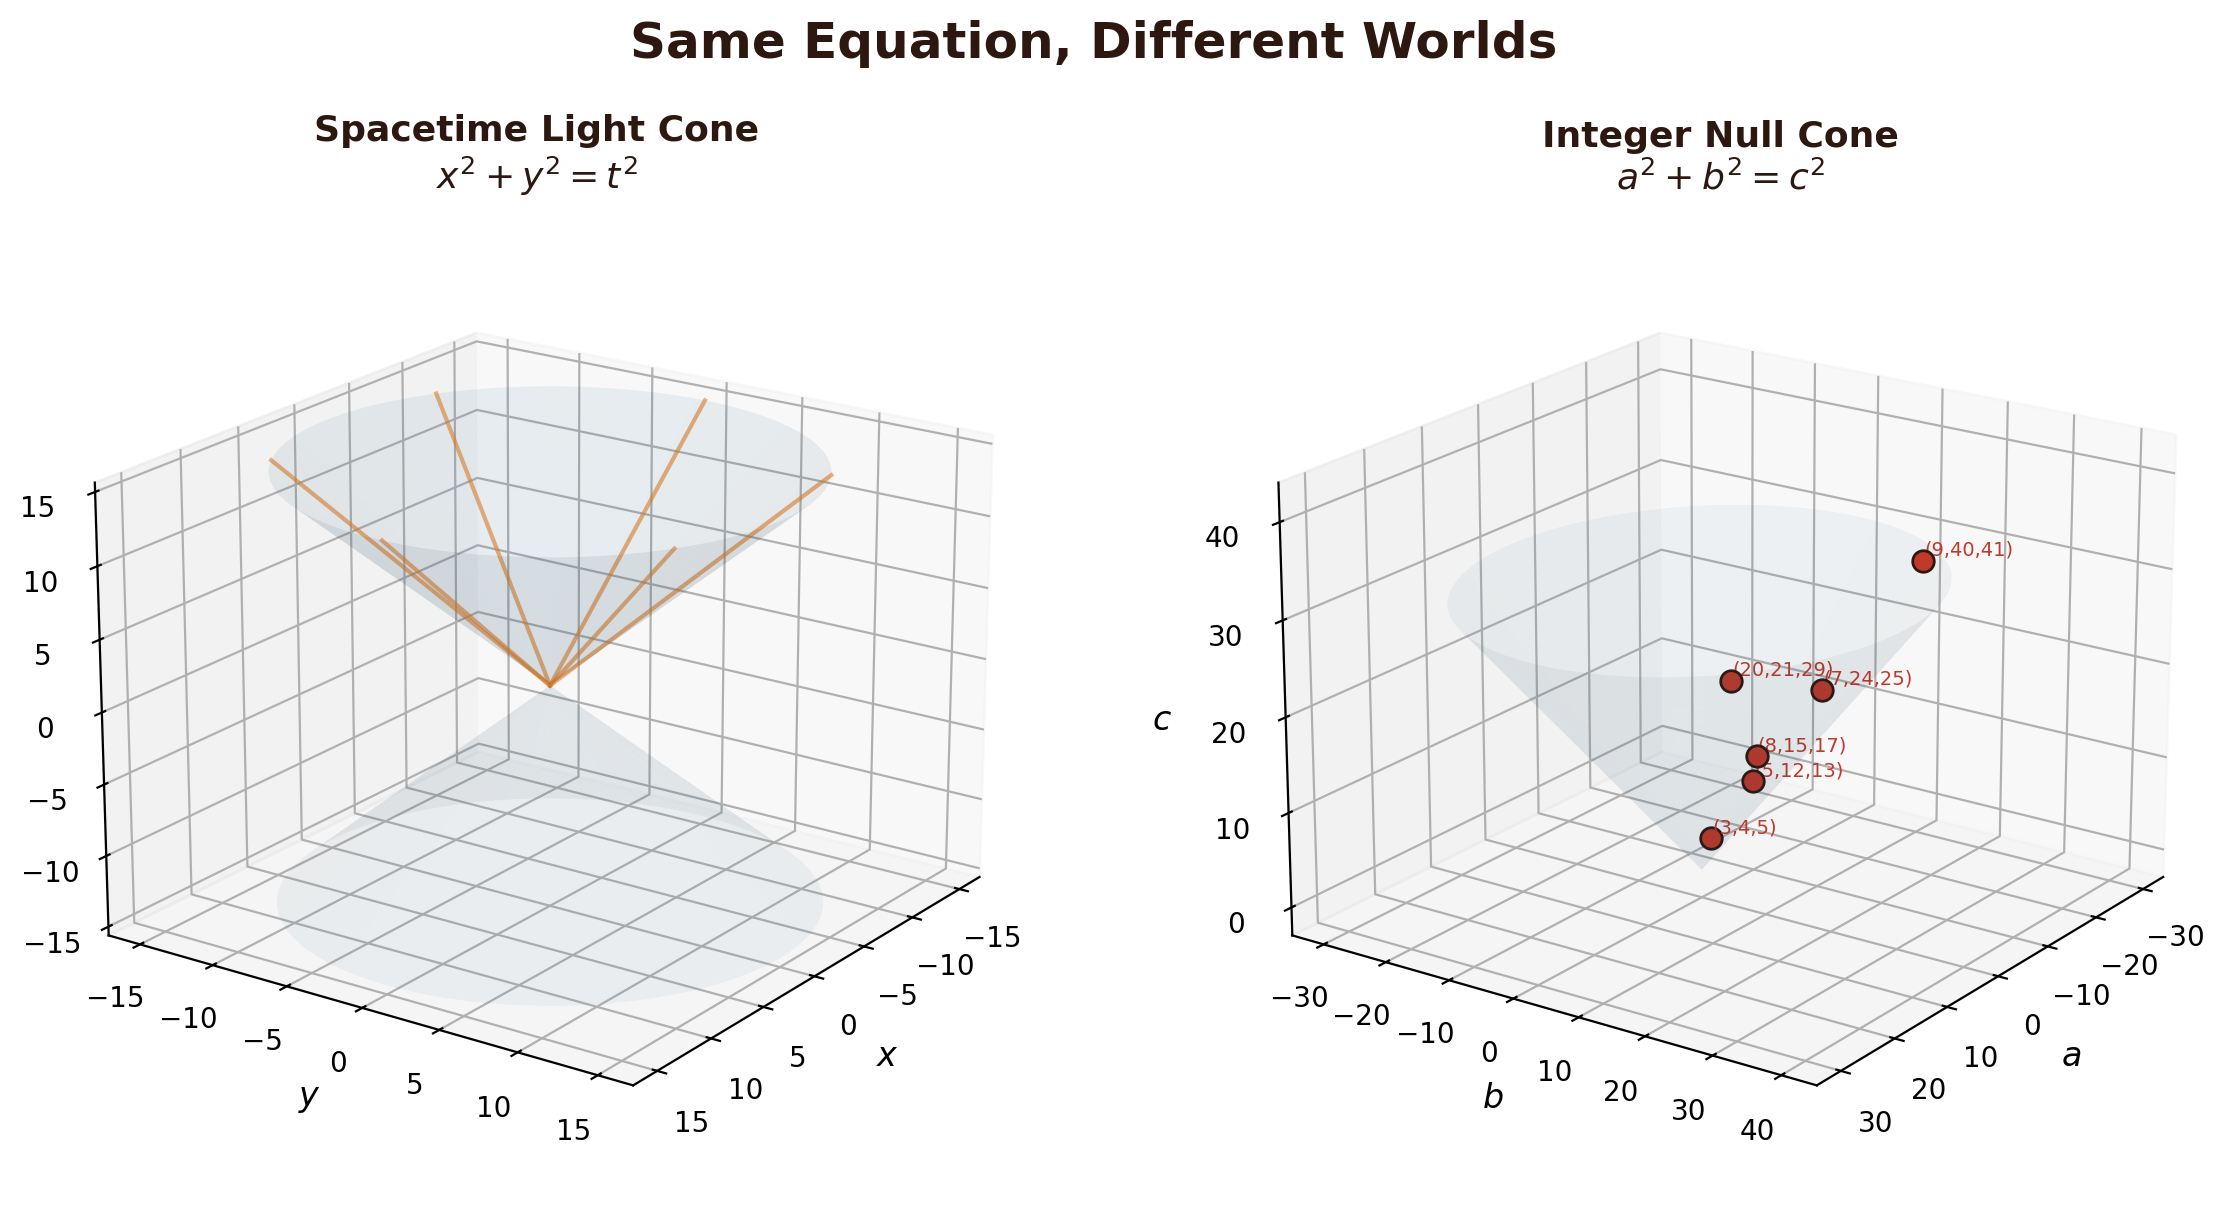
\includegraphics[width=0.75\textwidth]{../Chapter1/images/fig12_light_cones.png}
\caption*{Light Cones}
\end{figure}

\index{Cracking Numbers with Triangles}


Here is a number: $667$. It is not prime, but it \textit{looks} prime --- it passes many casual tests. Can you factor it? Probably not in your head. But I can hand you the factorization in seconds, \textit{using a right triangle}.\index{factorization}

The Pythagorean triple $(667, 156, 685)$ --- check: $667^2 + 156^2 = 444889 + 24336 = 469225 = 685^2$ --- gives us the identity

\[(c - b)(c + b) = c^2 - b^2 = a^2.\]

So $(685 - 156)(685 + 156) = 529 \times 841 = 23^2 \times 29^2$. Therefore $667^2 = 23^2 \times 29^2$, and

\[667 = 23 \times 29.\]

Done! The right triangle cracked the number like a nutcracker cracks a walnut.


This is no mere parlor trick. The factoring identity $(c-b)(c+b) = a^2$ is intimately related to Fermat's classical method of factoring by difference of squares. What the Berggren tree adds is \textit{structure}: instead of searching blindly for a representation $N^2 = c^2 - b^2$, you can walk the tree looking for triples where $a$ is a multiple of $N$. The tree provides a map of the territory.\index{difference of squares}



\bigskip\centerline{\rule{0.5\textwidth}{0.4pt}}\bigskip



\section*{The Fast Lane}

\begin{figure}[htbp]
\centering
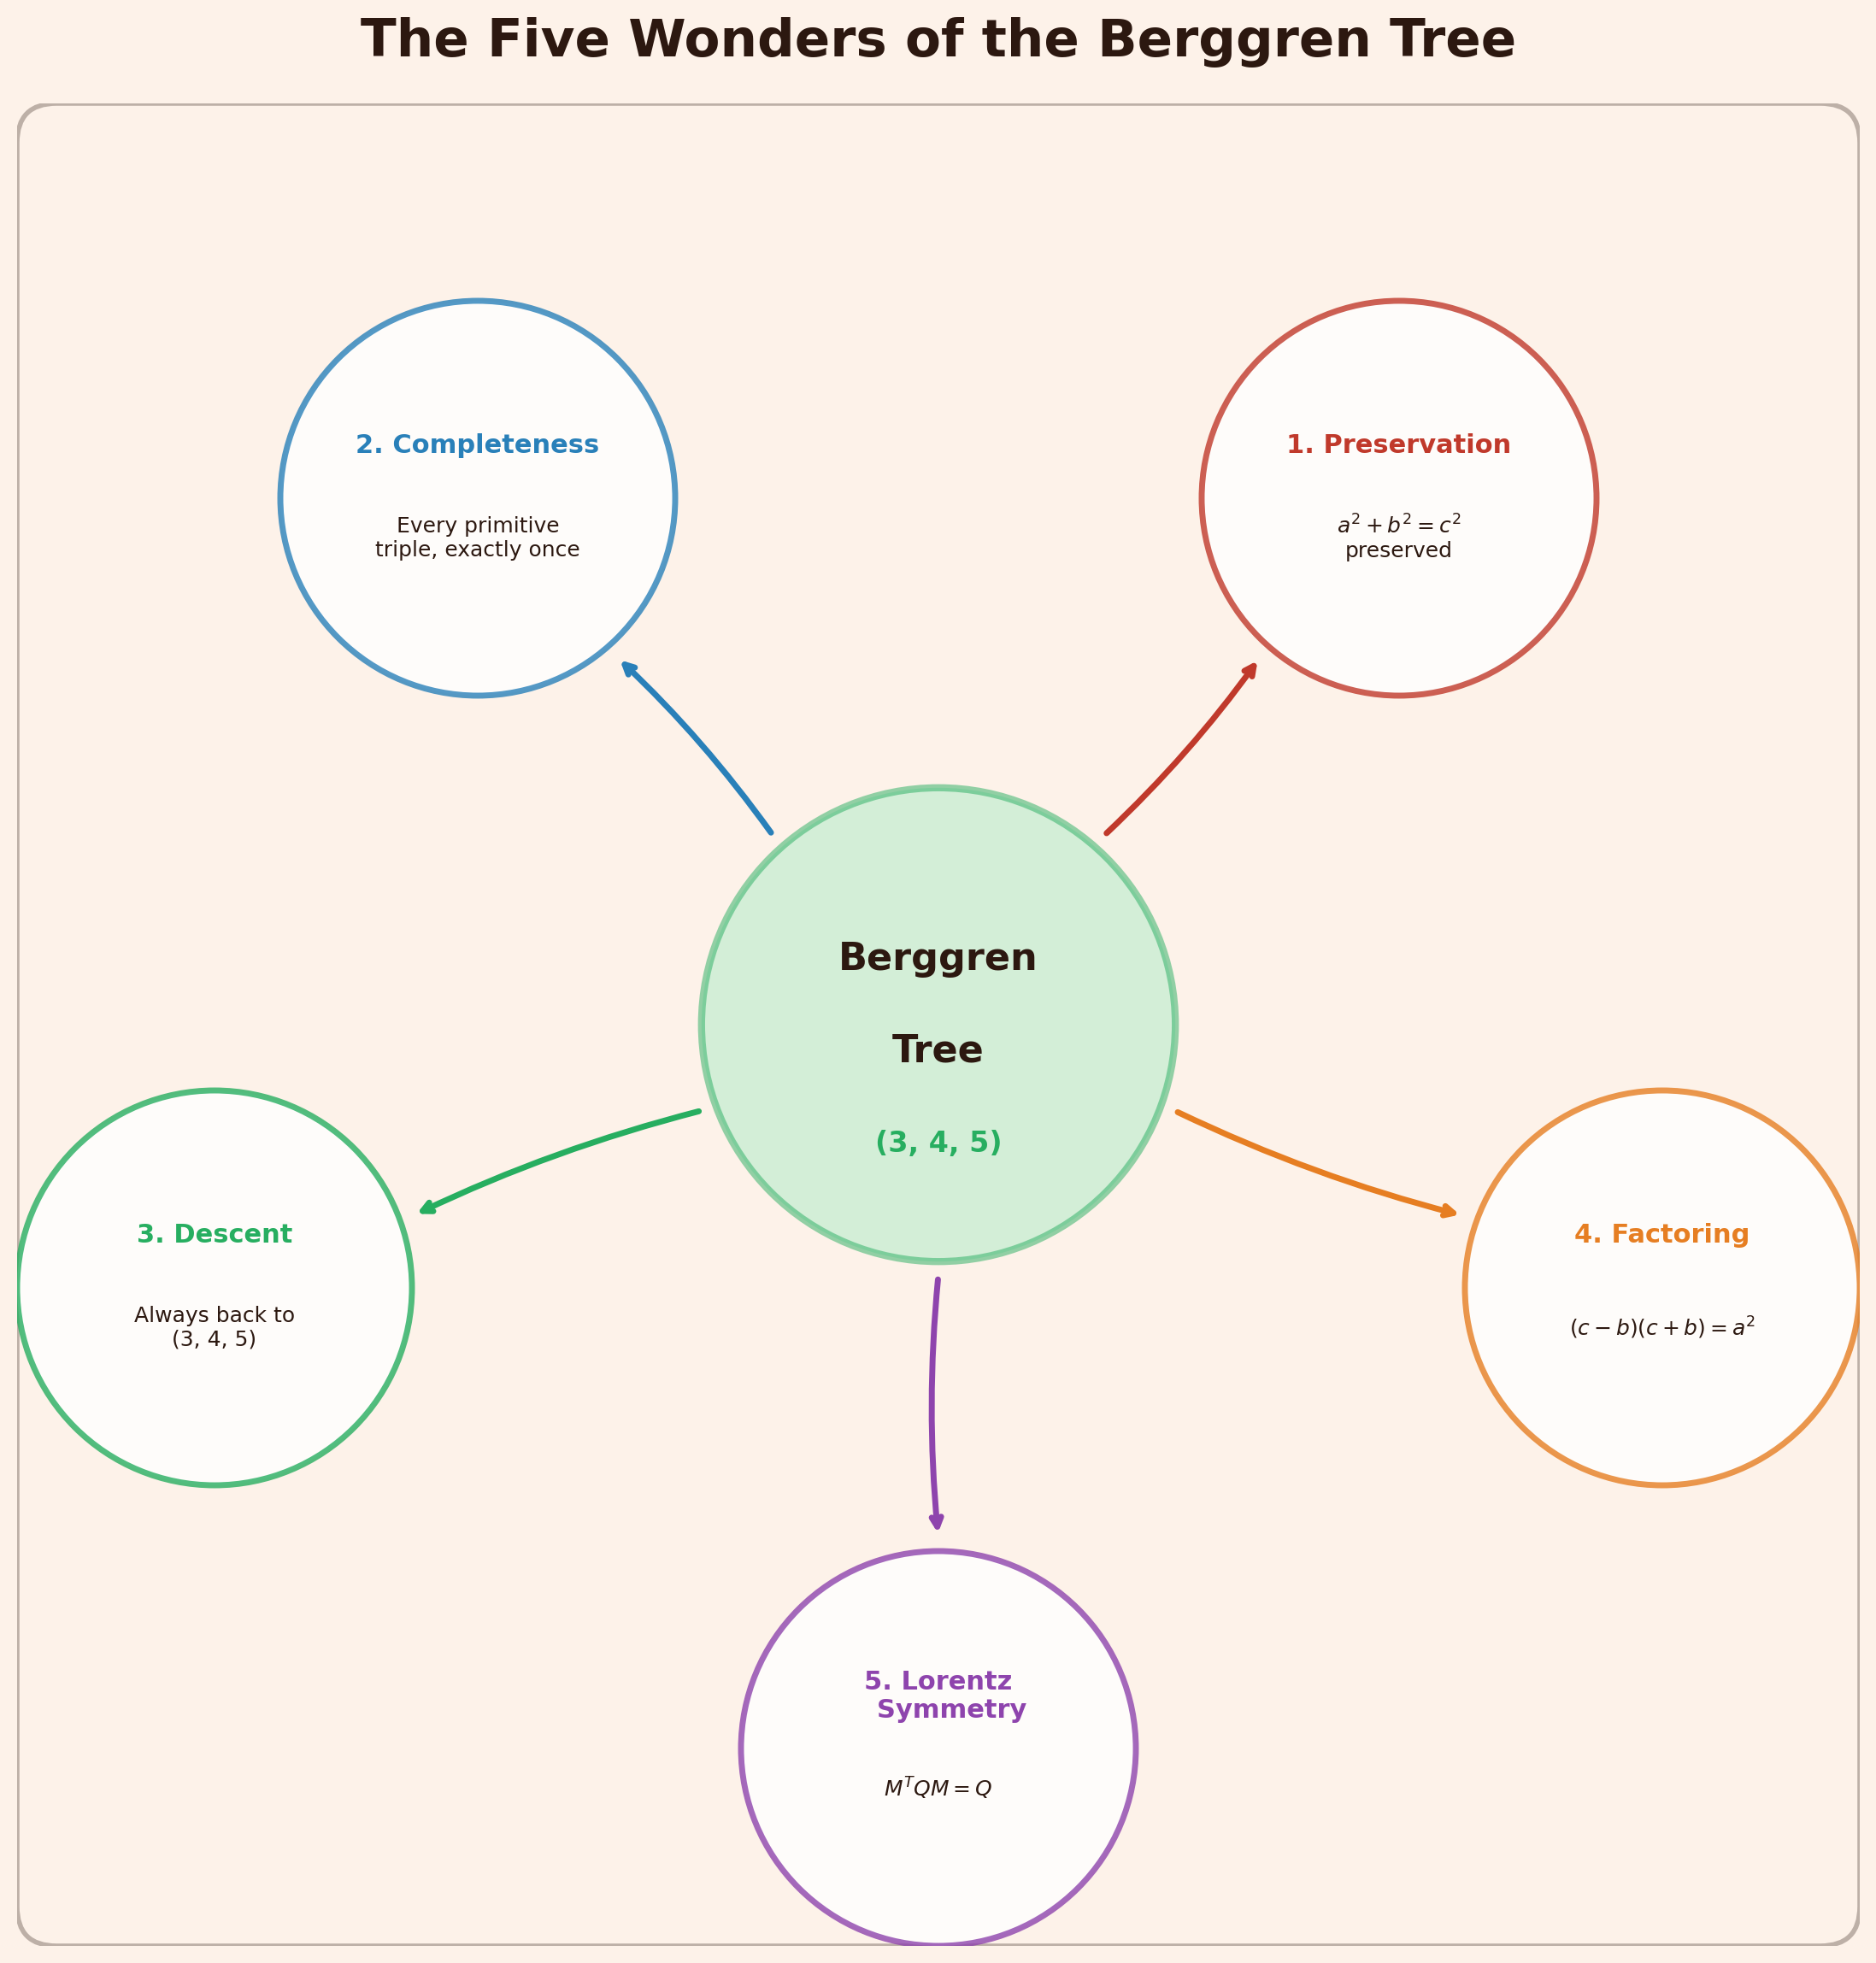
\includegraphics[width=0.75\textwidth]{../Chapter1/images/fig13_wonder_map.png}
\caption*{Wonder Map}
\end{figure}

\index{The Fast Lane}


Consider this sequence of hypotenuses: $5, 29, 169, 985, 5741, \ldots$ Each term is roughly six times the previous one, but not quite. Can you guess the rule?

The trick is to apply matrix $\mathbf{B}$ over and over, starting from $(3, 4, 5)$. The sequence of triples is

\[(3,4,5) \to (21, 20, 29) \to (119, 120, 169) \to (697, 696, 985) \to \cdots\]

and notice something enchanting about the legs: they always differ by one! $(21, 20)$, $(119, 120)$, $(697, 696)$ --- these are \textit{nearly isosceles} right triangles, and they grow ever closer to the $45$-$45$-$90$ ideal without ever reaching it.\index{ideal (ring theory)}

The hypotenuses satisfy a clean linear recurrence:\index{Lean 4}

\[c_{n+2} = 6\,c_{n+1} - c_n, \qquad c_0 = 5,\; c_1 = 29.\]

Check: $6 \times 29 - 5 = 169$. $6 \times 169 - 29 = 985$. $6 \times 985 - 169 = 5741$. The characteristic equation is $x^2 - 6x + 1 = 0$, with roots $3 \pm 2\sqrt{2}$. These are the fundamental units of the Pell equation $x^2 - 2y^2 = 1$ --- one of the oldest and most beautiful objects in number theory, misattributed to the English mathematician John Pell by Euler (who apparently confused him with Lord Brouncker, who actually solved it). Since $|3 - 2\sqrt{2}| \approx 0.172$, the second root shrinks to insignificance and the hypotenuses grow exponentially:\index{Pell equation}

\[c_n \sim \text{const} \cdot (3 + 2\sqrt{2})^n \approx \text{const} \cdot 5.828^n.\]



\bigskip\centerline{\rule{0.5\textwidth}{0.4pt}}\bigskip



\section*{Euclid's Ancient Engine}
\index{Euclid's Ancient Engine}


Over two thousand years ago, Euclid discovered a formula that generates Pythagorean triples the way a printing press generates pages. Give me any two positive integers $m > n$, and I will hand you a right triangle:\index{Euclid}

\[a = m^2 - n^2, \quad b = 2mn, \quad c = m^2 + n^2.\]

The proof that it works is pure algebra, requiring nothing beyond the identity

\[(m^2 - n^2)^2 + (2mn)^2 = m^4 - 2m^2n^2 + n^4 + 4m^2n^2 = m^4 + 2m^2n^2 + n^4 = (m^2 + n^2)^2.\]

Euclid's engine interacts beautifully with the Berggren tree. Consider the triples generated by \textit{consecutive} parameters, $n = m - 1$:


\begin{center}
\begin{tabular}{lll}
\toprule
$m$ & $n$ & Triple $(a, b, c)$ \\
\midrule
2 & 1 & $(3, 4, 5)$ \\
3 & 2 & $(5, 12, 13)$ \\
4 & 3 & $(7, 24, 25)$ \\
5 & 4 & $(9, 40, 41)$ \\
\bottomrule
\end{tabular}
\end{center}


These are exactly the triples along the $\mathbf{A}$-branch of the tree! Applying $\mathbf{A}$ to the triple from parameters $(m, m-1)$ yields the triple from parameters $(m+1, m)$. The matrix $\mathbf{A}$ is a "parameter escalator" --- it increments the Euclid parameters by one. Running it in reverse, $\mathbf{A}^{-1}$ steps \textit{down} the escalator, always converging back to $(2, 1) \mapsto (3, 4, 5)$.



\bigskip\centerline{\rule{0.5\textwidth}{0.4pt}}\bigskip



\section*{Spacetime Symmetry in Whole Numbers}
\index{Spacetime Symmetry in Whole Numbers}


In 1905, Einstein showed that the laws of physics are unchanged by Lorentz transformations --- symmetries that mix space and time while preserving the quadratic form $x^2 + y^2 - t^2$. Now look at what we have been doing all chapter: the Berggren matrices preserve $a^2 + b^2 - c^2$. They are Lorentz transformations --- integer ones.\index{Berggren matrices}

Formally, each matrix $\mathbf{M}$ satisfying $\mathbf{M}^\top \mathbf{Q}\, \mathbf{M} = \mathbf{Q}$ belongs to the group

\[O(2,1;\mathbb{Z}) = \{\mathbf{M} \in \mathrm{GL}_3(\mathbb{Z}) : \mathbf{M}^\top \mathbf{Q}\, \mathbf{M} = \mathbf{Q}\},\]

the \textit{integer Lorentz group}. Matrices with determinant $+1$ (like $\mathbf{A}$ and $\mathbf{C}$) are \textit{proper} Lorentz transformations --- orientation-preserving rotations of the null cone. Matrix $\mathbf{B}$, with determinant $-1$, includes a reflection; it is \textit{improper}.\index{Lorentz transformation}

The Berggren tree is, in the language of group theory, a \textit{Cayley graph} --- a map of the subgroup generated by $\mathbf{A}$, $\mathbf{B}$, and $\mathbf{C}$ inside $O(2,1;\mathbb{Z})$. And this subgroup tiles the hyperbolic plane, producing a tessellation that would have delighted M. C. Escher: an intricate, self-similar mosaic that grows finer and finer as you approach the boundary circle, each tile labeled with a Pythagorean triple.\index{hyperbolic geometry}




\bigskip\centerline{\rule{0.5\textwidth}{0.4pt}}\bigskip



\section*{The Five Wonders}
\index{The Five Wonders}


Let us step back and marvel at what a single $3 \times 3$ matrix equation has given us.

\textbf{Wonder 1 --- Preservation.} If $(a, b, c)$ is Pythagorean, then so are $\mathbf{A}(a,b,c)$, $\mathbf{B}(a,b,c)$, and $\mathbf{C}(a,b,c)$:
\[a'^2 + b'^2 = c'^2 \quad \text{whenever} \quad a^2 + b^2 = c^2.\]

\textbf{Wonder 2 --- Completeness.} Every primitive Pythagorean triple appears exactly once in the tree rooted at $(3, 4, 5)$.

\textbf{Wonder 3 --- Descent.} Every primitive triple can be traced back to $(3, 4, 5)$ in finitely many steps, because the hypotenuse strictly decreases under the inverse maps.

\textbf{Wonder 4 --- Factoring Bridge.} Each triple encodes a factorization via $(c - b)(c + b) = a^2$.\index{factoring}

\textbf{Wonder 5 --- Lorentz Symmetry.} The three Berggren matrices generate a subgroup of the integer Lorentz group $O(2,1;\mathbb{Z})$, and the tree is its Cayley graph, tiling the hyperbolic plane.\index{Cayley graph}


Five subjects --- number theory, algebra, geometry, physics, computation --- clasped hands in the branches of a tree that grows from a single seed: three knots, four knots, five knots, pulled taut on the banks of the Nile. If mathematics is the queen of the sciences, then the Berggren tree is one of her most elegant jewels.


\bigskip\centerline{\rule{0.5\textwidth}{0.4pt}}\bigskip



\subsection*{Puzzles for the Reader}


Before turning the page, try these on for size:


\begin{quote}
\itshape
\textbf{Puzzle 1.} Find all primitive Pythagorean triples with hypotenuse less than $30$.
\end{quote}



\begin{quote}
\itshape
\textbf{Puzzle 2.} Apply $\mathbf{A}$ to $(5, 12, 13)$. What do you get? Verify it's Pythagorean.
\end{quote}



\begin{quote}
\itshape
\textbf{Puzzle 3.} Starting from $(7, 24, 25)$, apply inverse matrices until you reach $(3, 4, 5)$. Which branch labels do you encounter along the way?
\end{quote}



\begin{quote}
\itshape
\textbf{Puzzle 4.} Use the difference-of-squares trick to factor $1073$. \textit{(Hint: find a Pythagorean triple with $a = 1073$.)}
\end{quote}



\begin{quote}
\itshape
\textbf{Puzzle 5.} Compute $c_4$ and $c_5$ using the recurrence $c_{n+2} = 6\,c_{n+1} - c_n$, starting from $c_0 = 5$ and $c_1 = 29$.
\end{quote}



\begin{quote}
\itshape
\textbf{Puzzle 6.} Which Euclid parameters $(m, n)$ produce the triple $(119, 120, 169)$?
\end{quote}



\bigskip\centerline{\rule{0.5\textwidth}{0.4pt}}\bigskip


\textit{But we have only begun. In Chapter 2, we shall discover that this tree hides inside a} lattice \textit{--- and that lattice will lead us deeper into the art of breaking large numbers apart…}\index{lattice}
